\documentclass{article}
\usepackage{amssymb}
\usepackage{geometry}
\usepackage{graphicx}
\usepackage{placeins}
\usepackage{hyperref}
\usepackage{xcolor}

\geometry{
	a4paper,
}

\title{Ingegneria del software II}
\author{Pierciro Caliandro}
\date{}
\begin{document}
\maketitle
\Large
\tableofcontents
\section{Modulo I - Machine Learning for Software Engineering}
\section{Ripasso: introduzione a SVN e Github}
Un sistema di controllo delle versioni tiene traccia dei cambiamenti ad un file ed inoltre permette di tornare indietro nelle versioni. Ci sono due tipologie:
\begin{itemize}
\item Centralizzata: SVN, utenti condividono una repository che è su un solo server centralizzato
\item Distribuito: Git, ognuno ha una copia della repo.
\end{itemize}
Differenze con classici sistemi di storage cloud sono varie:
\begin{itemize}
\item SVN e Git sincronizzano solo se c'è richiesta, mentre per sistemi cloud avviene in automatico
\item I merge sono a grana fine per SVN e Git, per Dropbox/Drive è a grana più spessa.
\item La storia delle versioni è mantenuta da SVN e Git, mentre poterebbe non esserlo per Dropbox/Drive
\end{itemize}
Working copy: versione su cui è possibile lavorare in locale. Non si lavora mai sulla risorsa condivisa, bensì su quella locale. \\ Revisione: particolare stato della risorsa condivisa, su cui è possibile tornare indietro. La versione è spesso una revisione particolare, che può essere offerta agli utenti (es versione 1.0 può corrispondere alla revisione 150).
\subsection{Issue tracking systems}
Sistema che permette di creare, assegnare e tenere traccia dei problemi (issues). Tutto nasce da Bugzilla (per progetti open source), un bug in un codice è molto simile a descrivere un requisito: nasce il concetto di ticket. Un ticket è un informazione rilevante al progetto, come un requisito da implementare o un bug.\\ Molti sistemi sono gestiti attraverso i ticket (medie-piccole dimensioni), ogni ticket ha un workflow: creato, assegnato, sviluppato, testato, approvato, chiuso. Tra gli esempi di sistemi per issue tracking ci sono Jira, Github, Redmine.
\section{Tecniche di Machine Learning ed analisi software a supporto della quality assurance e del testing}
I bug software costano circa 2.84\$ dollari ogni anno. Il codice viene scritto in diversi linguaggi, da tantissime persone, per poter fixare bug, aggiungere nuove feature e migliorare la qualità del codice. Il software è rilasciato con grande velocità, si vuole prevenire di avere bug in modo da avere technical debt basso.\\ Failure: comportamento osservato dall'utente e che non corrisponde alle specifiche del sistema. Un difetto software è quella parte di codice che può dare luogo ad una failure, questo non avviene sempre, ma solo sotto determinate condizioni. Per evitare le failure si cerca di individuare i bug prima che questi possano essere eseguiti dagli utenti.\\ È importante capire, avendo tempo limitato, come poter priorizzare le risorse di analisi. Si parla di software analytics come analisi di dati che riguardano progetti software.\\ Un aspetto importante è ML per poter predire ed evitare i bug futuri. In generale:
\begin{itemize}
\item Misuro i dati
\item Analizzo i dati e creo il modello di ML
\item Identifico quale classe/metodo è buggy
\end{itemize}
I dati sono gestiti da i version control systems ed issue tracking systems.\\ Importanti i commenti dei commit: invece di descrivere la modifica effettuata, faccio riferimento al ticket sul sistema. Dovrebbe esserci una relazione 1-a-1 tra ticket e commit: prendo il ticket e lo sviluppo per intero, in modo poi da fare il commit delle mie modifiche.\\ Se ho il tracciamento preciso tra ticket e codice che ho implementato per quel ticket, posso vedere se l'ammontare di linee di codice richieste per realizzare il ticket è maggiore o minore di quelle richieste per rimuovere il bug. Posso differenziare i ticket in base a bug e requisito e vedere il numero di righe cambiate.\\ Una volta estratti i dati, posso collezionare molte metriche a riguardo:
\begin{itemize}
\item Quante righe di codice modificate
\item Chi le ha modificate
\end{itemize}
\subsection{Metriche per individuare bug}
Posso usare metriche per fare delle stime su quale classe è buggy:
\begin{itemize}
\item relative al codice: classe con molte righe è potenzialmente buggy
\item processi: se file è stato affetto da molti cambiamenti
\item fattori umani: se file è stato toccato da sviluppatori esperti o non.
\end{itemize}
Posso leggere tutte queste info tal ticket di JIRA, ogni commit avrà un suo identificativo.\\ Si cerca di andare a capire quali file di una release sono defective o non defective. Avrò quindi dei dati che darò in pasto a modelli di machine learning black-box, con cui potrò capire dato un nuovo file quanto questo sarà defective.
È anche importante capire perché un file è difettoso, ci sono anche regole di normativa per cui se si usa una predizione bisogna anche fornire il perché della predizione. È possibile anche vedere il perché una classe ha avuto una certa probabilità di essere difettoso.
\subsection{Process control chart}
Chart che mostra la stabilità degli eventi nel tempo: è importante che sull'asse verticale ci sia l'elemento di cui si vuole controllare la stabilità, mentre sull'asse orizzontale ci deve essere qualcosa che possa essere misurato.\\
Voglio vedere se un certo progetto ha dei difetti per in base al numero di revisione: metto su asse x il tempo (es settimane, o le revisioni), asse y avrò i difetti. Mi chiedo se in un progetto i difetti sono lineari in base alle revisioni. Dobbiamo:
\begin{itemize}
\item Selezionare i dati sull'asse y ad esempio il numero di commits o requirements 
\item Seleziono dati per asse x, asse temporale. Può essere giorni/mesi o anche release
\item Colleziono i dati
\item Calcolo media e varianza, imposto poi degli assi di limiti superiori ed inferiori (ad esempio):
\begin{itemize}
\item limite superiore (upper control limit): media + $3\cdot$deviazione standard
\item limite inferiore (lower control limit): media - $3\cdot$deviazione standard. Può andare sotto 0, alle volte conviene andarci ma altre volte no (quindi lo si fa fermare a 0).
\end{itemize}
\end{itemize}
Visualizzando il chart, posso capire se qualcosa è andata particolarmente male: quando un punto è al di fuori del limite, è significativamente diverso da tutti gli altri punti. Quindi in questo caso si analizza il perché per una determinata release c'erano dei valori così estremi, ad esempio perché c'è stato un numero così elevato di difetti.
\subsection{Ripasso: continous integration e travis}
Pratica per cui i membri del team integrano il loro lavoro continuamente. Ogni integrazione è verificata con un build del progetto, viene fatto per evitare errori nell'integrazione del progetto.\\ È molto importante che il built sia automatico, in modo che chiunque possa effettuarlo, e non solo alcuni membri del team. Importante anche che la built sia self-testing, e che inoltre i commit avvengano quotidianamente o almeno per ogni feature.\\ I test vanno effettuati in un ambiente che sia il più possibile simile all'ambiente di production: ad esempio, se ho sviluppato un app, il production environment sarà il dispositivo dei miei utenti.
\subsection{Ripasso: technical debt}
Applicazione di concetti finanziari al dominio del software engineering. Code smell e regole di qualità: una regola di qualità è un principio che detta come il codice dovrebbe essere, ad esempio:
\begin{itemize}
\item alta densità di commenti
\item bassa densità di codice
\item if statement non difficile da leggere
\end{itemize}
Una violazione o code smell è una porzione di codice non perfetto. È importantissimo soffermarsi sulla differenza fra difetto e code smell: difetto può dare vita ad un failure (sotto determinate condizioni), mentre il code smell è qualcosa non osservabile dall'utente (ad esempio la lunghezza di un if statement). Il problema è che i code smell impattano gli sviluppi futuri.\\ Il debito tecnico può essere visto come un qualcosa che darà problemi a sviluppi futuri (impatta la prossima release), può emergere organicamente come molti sistemi aumentando di complessità, aumentano la loro complessità di gestione. Inoltre, può anche essere scelto in maniera opportunistica, ovvero decidere deliberatamente di avere una certa quantità di debito tecnico.\\ Il technical debt consiste in due parti:
\begin{itemize}
\item principio: costo per eliminare i code smells
\item interesse: la penalità da pagare in futuro per il debito non eliminato
\end{itemize}
Come gestisco i code smell attraverso i ticket: tutto ciò che bisogna fare deve essere scritto in un ticket. Non c'è altro mezzo di informazione che il progetto può usare, linee guida e processi aziendali possono essere documentati su un altra piattaforma (confluence, per completare JIRA).Se c'è un code smell, \textbf{dipende dal processo aziendale}: può essercene uno che dice che chi ha introdotto lo smell lo toglie senza ticket, un altro che dice che i problemi rilevati da Sonar Cloud verranno analizzati a parte da specifiche persone che avranno il ruolo di aprire i ticket appositi. È possibile impostare i repository in modo che rigetti i commit che violano alcune regole di qualità (configurando Travis/Jenkins), così saprò che il codice è sempre smell free.
\subsection{Misure di analisi}
Voglio rispondere alla domanda: le linee di codice per le feature, sono state di più o di meno di quelle usate per risolvere i bug? Quando gestisco i dati, posso farlo per due motivi:
\begin{itemize}
\item guardare al passato: perché spendo molte LOC per risolvere i bug? Vado a fare delle analisi introspettive sul progetto
\item avvento del ML, predico il futuro: prendo delle decisioni nel presente, in modo che l'impatto dei cambiamenti futuri sia controllato
\end{itemize}
\section{Merging JIRA con Git}
\subsection{Git: comandi utili}
Una volta effettuato il clone di una repository, è possibile avere accesso al log: \textbf{git log $<$options$>$}, da accesso ai cambiamenti mostrando
\begin{itemize}
\item autore del commit
\item cambiamento
\item commento 
\end{itemize}
se non viene specificato il branch, git ritorna il log di quello corrente. Una cosa interessante può essere comparare due commit fra loro, per vedere i cambiamenti: tramite il comando \textbf{git diff $<$commit\_id$>$..$<$altro commit\_id$>$}. Alcune visualizzazioni sono human readable, ma nel codice che fa l'analisi automatica non è importante.\\
Data la revisione di un file, per ogni riga è possibile risalire al commit che ha inserito quella determinata riga: ho un file di 10 righe, mi chiedo chi ha inserito una riga, quando e perché. \textbf{git blame $<$filename$>$} (con -w ignora gli spazi bianchi). Fornisce la data dell'ultima modifica con la relativa modifica (ci sono anche meccanismi per andare indietro) e chi l'ha effettuata. È possibile fare il grep sul testo, in modo da cercare solo specifiche parti di interesse del log.
\subsection{Cercare ticket in JIRA}
Una volta trovato un progetto, è possibile selezionare il tipo di ticket da cercare, lo sviluppatore etc... (numerosi filtri), in advanced è anche possibile creare delle query SQL-like, con cui è possibile creare delle ricerche sofisticate e metterle da parte.
\section{Snoring and proportion}
Quando vedo un commit per un ticket di tipo bug, che ha toccato 3 classi, so che quelle 3 classi prima del commit erano buggate prima del commit. Con il blame so qual è il commit preciso che ha prodotto un determinato stato di una riga. In generale, la predizione dei difetti cerca di individuare quale artefatto software è più propenso a mostrare difetti: ci mettiamo nei panni di chi deve testare la release finale (molte classi) per capire quale classe è opportuno testare. Vorremmo una stima di quanto una classe è probabilmente buggy, per ordinarle in modo crescente (per probabilità).\\ Prima di poter fare delle stime, è necessario misurare cosa stimare: quando si fa una predizione: un conto è farla binaria, un altro è se vanno predetti dei numeri. Quest'ultima è estremamente più complessa di quella binaria.\\ esempio: supponiamo di dover predirre il meteo, a seconda del fatto che io dica che piove o no, o che piove 20 cl. Non ho alcune informazioni, ad esempio se piove più o meno di 20 cl o in media 20 cl. Potrei avere predizioni diverse per giorni diversi. Bisogna fornire \textbf{un grado di confidenza} (e quindi intervallo di confidenza), in modo da rendere la previsione più comprensibile. L'approccio del Machine Learining consiste nell'utilizzo dello storico dei dati: ad esempio per il meteo posso avere delle misure storiche che mi aiutano a stimare le previsioni per un determinato giorno, in base a misure passate che hanno avuto lo stesso risultato conseguente. Quindi per predirre il comportamento di una classe in futuro, devo poter conoscere il suo comportamento passato e quindi le misure passate.\\ Il progetto è un insieme di classi, ho varie revisioni e varie release (o versioni): alcune classi evolvono durante il tempo, che è diviso in versioni, ed ogni tot revisioni (che corrisponde ad un commit) ho delle release.
\subsection{Difetti dormienti}
Per definire un classe difettosa, questa deve contenere un bug. Il problema è che per capire se una classe è o meno difettosa bisogna avere come input i bug: in base a questo, troviamo il commit che ha eliminato il bug, che tocca delle classi che quindi erano bug. È possibile che un difetto sia scoperto ed eliminato diverse release dopo la sua introduzione: è stato introdotto nella release 1.0 ed eliminato nella 3.2, ma quando ero in release 3 non avendo fatto il fix del bug non ne conoscevo l'esistenza e non conoscevo le classi che lo contenevano.\\ L'esistenza di un difetto non può essere nota prima che questo sia eliminato, abbiamo diverse versioni.\\
\includegraphics[scale=0.4]{images/AV-isw2.png}\\
le affected version (AV) sono quelle affette dal bug, la AV è definita come la injected version (IV) inclusa e la fixed version (FV) esclusa, ho anche la open version (OV), ovvero quando il ticket è stato aperto. Il problema è capire qual è la IV, ovvero quando il bug è stato introdotto.\\
Se ho creato il ticket in un certo intervallo temporale, non sapevo quale classe aveva bug. Abbiamo un commit, che ha come commento il fix di un bug relativo ad un ticket e possiamo scoprire quale riga aveva un bug; inoltre, sappiamo che la versione successiva a questa non abbiamo più il bug.\\ Ci accorgiamo di due problemi:
\begin{enumerate}
\item se non avessimo cambiato la riga di codice, non avremmo mai scoperto che la classe aveva un bug e quindi fino a quel periodo temporale ci sembrava che la classe fosse bug free.
\item supponiamo che la versione successiva non sia buggy, il problema è sapere quando questo bug è stato iniettato: sappiamo che la classe aveva un bug e adesso non lo ha più, ma non so per quante revisioni/versioni passate la classe aveva il bug
\end{enumerate}
per poter fare delle stime occorre conoscere tutte le revisioni in cui la classe era buggy, dobbiamo poter andare indietro nel tempo per poter etichettare la classe come buggy finché serve. Quindi, usando il \textbf{blame}, posso scoprire quale commit ha introdotto il bug e posso anche scoprire in quale versione ricade il commit ed in quale versione viene risolto. Per ogni commit ho una data: se so che le versioni sono ordinate temporalmente (ad esempio se so che ogni tot viene rilasciata una versione) posso sapere, in base alla data del commit, a quale versione appartiene, in quale versione era buggy e quando no
\subsection{SZZ}
Metodo che consiste nell'usare il \textsf{blame} per capire qual è la prima versione in cui il bug è stato introdotto. Andiamo indietro nelle versioni, fino a trovare quando la LOC buggy è stata creata, un altro approccio è quello di vedere le AV in Jira: quando l'utente elimina il bug, fa anche una stima di quali versioni erano affette dal bug, quindi possiamo leggere i ticket Jira, in particolare il filed, ma non è detto che ci sia.
L'approccio ha comunque dei problemi: 
\begin{itemize}
\item se per introdurre una feature cambio qualcosa che funzionava ed ora non funziona più, sono costretto a cambiare quello che funzionava, ed SZZ mi direbbe che il bug è nella classe che funzionava, ma prima di introdurre la feature il problema non c'era, ovvero introduco un regression bug\footnote{facendo una modifica di una parte di codice, andiamo a rompere un'altra parte di codice, senza rendercene conto, in quanto non possiamo testarla}.
\item il blame va una sola volta indietro e non sappiamo quante volte occorre andare indietro (anche se è possibile settare fin quando andare indietro)
\item se dei cambiamenti in realtà non aggiungono nulla (ad esempio refactoring di codice) possono essere colpiti dal blame, quando in realtà la modifica è non funzionale. Ci sono tool che vanno indietro finché non trovano una modifica funzionale, scartando quelle non funzionali
\end{itemize}
Per poter predirre il futuro, devo utilizzare i dati del passato: ci stiamo orientando per poter predirre quali classi sono buggy, deve essere possibile quali erano buggy.
\subsection{Prediction dataset}
La predizione di difetti cerca di identificare gli artefatti software che hanno dei difetti, lo scopo è quello di ridurre l'effort di testing e code review. L'affidabilità della predizione dipende dalla qualità dataset, esistono diversi sorgenti di rumore nel dataset (in-accuratezze), ad esempio la mail classificazione dei difetti, ovvero difetti taggati in Jira che non lo sono, o anche la difficoltà di andare indietro col blame etc... È possibile predirre:
\begin{itemize}
\item commit
\item classe
\item altro
\end{itemize}
e dire se questi sono buggy. Il nostro contesto sarà predirre la buggyness di una classe, avranno delle probabilità assegnate. La stessa classe appare in diverse revisioni e diverse release: ci mettiamo nei panni di chi è all'ultima revisione e vuole testare lo stato della classe prima di fare la nuova release. Il problema di capire l'origine dei difetti è che alcuni difetti possono essere scoperti solo dopo che sono stati introdotti: esistono difetti che vengono introdotti e risolti nella stessa release, marchiamo con:
\begin{itemize}
\item I: difetto iniettato
\item F: difetto fixato
\item N: nulla
\end{itemize}
è possibile inserire più di un difetto in una release\\\\
\begin{tabular}{ |c|c|c|c|}
\hline
 & $r_1$ & $r_2$ & $r_3$\\
\hline
$C_1$ & IF & N & F\\
\hline
$C_2$ & I & N & F\\
\hline
$C_3$ & II & F & F\\
\hline
\end{tabular}\\\\
Può accadere che sono in una release in cui non ho fatto il fix di un difetto introdotto in quella precedente, quindi non ne conosco l'esistenza. Quindi, quando parte il balme, questo mi classifica la classe come non buggy. Tutte e tre le classi della tabella, in release 2 sembrerebbero non buggy se la misurazione venisse fatta in release II, diverso se fatta nelle altre release: quindi, cambia lo stato a seconda di quando avviene la misurazione.\\ Più la release è recente, più c'è il problema che alcune classi mi sembrano non buggy anche se lo sono. Quindi, è più probabile che le release abbiano dei bug dormienti: se sono in release i, le ultime mi sembrano tutte non buggy, perché magari li troverò dopo mesi. C'è il problema di capire se si possono usare i dati di queste release. Il numero di bug nelle release è decrescente, in quanto c'è il problema dei bug dormienti; la predizione fa sempre riferimento alla coppia (classe, release), NON VANNO CONSIDERATI QUELLI PRECEDENTI
\subsection{Snoring}
Concetto importante nella misurazione dei difetti nelle classi: ho positivi e negativi, il positivo è la classe buggy. Parlo di falso positivo quando la classe mi sembra buggy e non lo è. Il problema è un falso negativo, in quanto la classe mi sembra non defective, quando in realtà lo è. Questo perché la misurazione avviene (ad esempio tramite SZZ) considerando i bug non ancora eliminati.\\ Una classe è snoring se la classe ha uno o più bug di tipo dormiente, una classe in realtà è snoring se sembra non buggy,ma in realtà lo è.\\ Con riferimento alla tabella sopra, nella release 1 le prime due classi mi sembrano non defective, la classe 3 mi sembra defective, in quanto per fare la misurazione sto nella release successiva, quindi avendo un fix la release precedente mi sembra defective.\\\\
\begin{minipage}[t]{0.5\textwidth}
\begin{tabular}{ |c|c|}
\hline
Classes & $r_1$\\
\hline
C1 & ND\\
\hline
C2 & \textbf{ND}\\
\hline
C3 & D\\
\hline
\end{tabular}
\end{minipage}%
\begin{minipage}[t]{0.5\textwidth}
\begin{tabular}{ |c|c|c|c|}
\hline
Classes & $r_1$ & $r_2$\\
\hline
C1 & ND & D\\
\hline
C2 & \textbf{D} & D\\
\hline
C3 & D & D\\
\hline
\end{tabular}
\end{minipage}%
\\\\
Domande di ricerca che provano a capire:
\begin{itemize}
\item per quanto tempo le classi "dormono"
\item per quanto tempo le classi sono snoring
\item lo snoring impatta la misura delle stime fatte?
\end{itemize}
Vogliamo vedere quante release passano in media dall'injection al fix: per ogni bug, per quante release questo è dormiente.\\
\\ la linea centrale rappresenta la mediana, quindi possiamo dire che la maggior parte dei difetti in \textit{Connectors} ha dormito per almeno 25 release.
\\ qui abbiamo la percentuale (delle release di sleep). Quindi, se non volessimo il rumore nei dati, dovremmo scartare questa percentuale di release (altrimenti me perderei quei bug, che sono dormienti).\\ Se io misuro la buggyness di una classe, il fatto che alcuni bug dormano non è un problema, l'importante è trovarne almeno uno per far si che la misurazione sia corretta.
\subsubsection{Misurare lo snoring}
Supponiamo di avere un tot di release, considerarle tutte farà si di avere un certo livello di snoring, soprattutto nelle ultime: meno ne considero, meno snoring avrò ma serve avere un compromesso rispetto alla taglia del dataset, quindi non è possibile dare massima priorità all'accuratezza del dataset.\\ Quindi, dobbiamo misurare come cambia l'accuratezza in base alle release tolte: per capire come l'in-accuratezza varia al variare del tempo, il \textit{missing rate} è la percentuale di classi che sono falsi negativi diviso tutte le classi positive, ovvero $\frac{FN}{FN + TP}$, la percentuale di classi positive che perdo nella misurazione.\\ Per capire se varia nel tempo, devo vedere quando un set di bug vengono trovati nel tempo: se prendessi le prime release, avrei un certo grado di inaffidabilità rispetto a quelle ancora prima, devo vedere quando sono stati trovati i primi bug, quindi mi soffermo sul primo 5\% del dataset. Misuro cosa accade al primo 5\%, misurato con diversi punti di osservazione, che variano nel tempo (misurato col numero di release), ovvero come cambia lo stato delle classi se le osservassi in futuro.\\ Quindi, in base al missing rate, so quante release devo scartare: ad esempio, per la  maggioranza delle release, il missing rate è più del 50\% a meno che non venga tolto il 20\% delle release.
\subsubsection{Impatto dello snoring sull'accuratezza della perdizione}
Ci son due concetti importanti in Machine Learing:
\begin{itemize}
\item training set: dati con cui viene costruito il modello
\item testing set: dati che vengono usati per misurare la correttezza del modello
\end{itemize}
una parte dei dati non verranno usati (unused data). L'accuratezza della stima, sullo stesso modello migliora considerando le release sempre più avanti nel futuro, ma non è possibile aspettare troppo. Lo step successivo è chiedersi, dato che si sa che lo snoring cresce al crescere delle release, se il modello non prende in considerazione le ultime release migliora la qualità della perdizione, ovvero avere meno dati è meglio che avere dati con snoring: l'ultima release da dei dati talmente snoring che è conveniente non usarla, ma dipende dal tipo di modello che si usa: dipendentemente dal fatto che si vuole aumentare la precisione di uno o più modelli, occorre togliere più o meno release. Esistono poi classificatori che sono più o meno robusti allo snoring.\\ Ultime considerazioni
\begin{itemize}
\item togliere una release è sempre meglio che non toglierne per l'accuratezza
\item rimuovere 3-4 release è sempre peggio che toglierne una
\end{itemize}
rimane come questione se toglierne una o due.
\subsubsection{Rimozione di release dal dataset}
Cosa succede se "fotografiamo" la situazione degli stessi dati in punti di vista (release) differenti: vediamo la situazione dopo il training set, e cerchiamo di stimare il testing set. A seconda della porzione di training set che osservo, avrò dei risultati differenti: voglio trarre delle considerazioni come ad esempio il modello o la tecnica più accurata per fare predizioni, mi occorrono quindi dei dati affidabili, per fare questo buttiamo l'ultima metà dei dati, che so che sono poco affidabili. Se voglio trarre delle conclusioni da un punto di vista scientifico, sono in una soluzione in cui non vedo snoring, è utile per fare ragionamenti sulla bontà del modello. Da un punto di vista pratico vado a considerare il training set in diversi punti  e quindi avrò un certo snoring nei dati.
\section{Leveraging defects}
Non usiamo SZZ, ma un altro meccanismo: si parte sempre dal presupposto che il bug sia stato versionato da un commit in Jira e che ci sia un ticket a riguardo. Una volta che sappiamo quale riga di codice è stata cambiata per risolvere un bug, sappiamo allora che quella era buggy. Ci sono però tutti i problemi introdotti con SZZ: un fix può essere dovuto ad un refactoring, inoltre occorre capire quali revisioni e versioni del codice erano buggy. Se non riusciamo a classificare una release come buggy o non buggy non posso creare il dataset per le stime.\\ La predizione dei difetti cerca di identificare gli artefatti software che esibiscono un difetto, il vantaggio è quello di ridurre il costo del testing e della code review.\\ Quindi, il lavoro si focalizza sulla creazione di un dataset per poter fare le predizioni. Per fare un ranking delle classi come defective o non: facciamo il \textbf{labeling} di una classe in una release, occorre identificare in maniera separata le due classificazioni:
\begin{itemize}
\item una avviene al momento della creazione del dataset
\item la classificazione per la predizione
\end{itemize}
una cosa è l'input (dati passati) del modello, un'altra sono gli outout del modello. Col labeling, identifichiamo classificazione di una classe come buggy o non buggy nel passato. Per farlo, possiamo usare SZZ oppure verificare nel ticket di Jira il campo di \textit{affected version}. Quando l'AV non è presente, l'unica tecnica era usare il blame ma qui c'è la difficoltà di capire quanto andare indietro
\subsection{Defect lifecycle}
Ciclo di vita di un difetto: rappresenta lo stato di un difetto:
\begin{itemize}
\item fixed version (FV): prima versione bug free, ci sarà un fix commit. Abbiamo le diverse revisioni e le versioni, il fix commit produrrà la prima versione senza bug, che è la FV
\item c'è una versione in cui è stato cerato il ticket: qualcuno ha identificato una failure, chiamo la versione con il ticket del bug aperto opening verison (OV). In Jira, so sempre quando un ticket è stato aperto e quando è stato eliminato
\item Injected version (IV): versione dove il bug è nato, non la conosciamo
\end{itemize}
per definizione, tutte le versioni aventi quel bug sono affected version (AV). La fixed version è sempre bug free, prima dell'injected version le versioni non hanno il bug; quindi tutte le versioni affected vanno dall'injceted (inclusa) alla fixed (esclusa).\\ Lo scopo è vedere la percentuale dei casi in cui l'AV è disponibile nei ticket, per capire quanto il problema è grave. Se non è disponibile, cerchiamo un metodo alternativo ad SZZ.
\subsubsection{Affected version in Jira}
L'IV deve essere antecedente alla OV, in quanto prima devo inserire il bug e poi formulare il ticket. Vediamo la percentuale dei ticket che hanno una AV disponibile e consistente (ovvero non antecedente alla OV): circa $\frac{1}{3}$ dei casi non ha l'AV disponibile nel ticket. Su un analisi di circa 125k bug, la maggior parte non aveva AV o la aveva non affidabile. Occorre capire quindi quale release della classe sono affected o no, supponendo che le AV non fossero disponibili.
\subsection{Metodo proportion}
L'assunzione è che i difetti hanno un ciclo di vita: più è grande la distanza fra IV ed OV\footnote{in termini di numero di versioni}, più è grande la distanza fra OV e FV. L'unica incognita è l'IV: ci basterebbe calcolare la proporzione nei bug dove sappiamo qual è l'IV ed utilizzare il risultato nei casi in cui l'IV non è disponibile (e quindi non sappiamo nemmeno l'AV).\\ La proporzione è  fissa: $P = \frac{(FV - IV)}{(FV - OV)}$, l'IV predetto sarà $IV = FV - (FV - OV)\cdot P$. Ci sono delle varianti per calcolare P:
\begin{itemize}
\item cold start: non ho dati passati, posso usare i dati di altri progetti. Calcolo la media dei P di altri porgetti e lo uso sul mio
\item incremento: calcolo P come la media dei difetti fixati nelle versioni precedenti (a bug 14, userò il P computato da 1 a 13). Il ciclo di vita del progetto può cambiare, quindi anche il ciclo di vita dei difetti. Usare quindi tutta la storia passata può non essere corretto
\item moving window: P viene calcolato come la media dell'ultimo 1\% dei difetti fixati, fa fronte al problema dell'approccio incrementale.
\end{itemize}
Assumiamo di non avere l'AV, come facciamo a stimare: sappiamo che l'AV è un insieme di versioni e la prima è sempre l'IV, quindi abbiamo diversi metodi di stima:
\begin{itemize}
\item simple: assumere che la prima IV è uguale a quanto il ticket è stato creato, ovvero OV; varianti di SZZ
\item proportional
\end{itemize}
Ci sono i concetti fondamentali:
\begin{itemize}
\item positivo (TP): la versione è misurata come difettosa e viene marcata come difettosa
\item negativo (TN): versione misurata come non difettosa ed etichettata come non difettosa
\item false positive (FP): versione misurata per essere non difettosa, ma etichettata come difettosa
\item false negative (FN): versione misurata per essere difettosa ma etichettata come non difettosa
\end{itemize}
Per la maggior parte dei classificatori, il metodo proportioning è migliore di SZZ, tranne che per la recall (molto affetta dai FP).\\ Qual è la relazione fra l'accuratezza della misurazione e quella della stima: nella predizione usiamo delle caratteristiche come dati di input, una volta creati i dataset per fare ciò, possiamo usarli per fare analisi di correlazione. Ci sono varie metriche che possono essere usate per relazionarle alla buggyness.
\paragraph{Linee guida generali:}se in un ticket di Jira ci sono buchi nelle AV (ad esempio non si sa cosa c'è nel mezzo) o tra AV e FV, si può procedere in questo modo: si imposta la IV come la prima AV e tutte quelle che $\in [IV, FV)$ sono AV.
\subsection{Problematiche nel mining Github}
Abbiamo visto come analizzare i difetti e prendere determinate decisioni. Github è attualmente la codebase più grande del mondo, quindi l'abbondanza dei dati semplifica il problema di collezione dei dati e del processamento. Le analisi possono essere scorrette, ci sono delle difficoltà che possono alterare le conclusioni se i dati sono stati analizzati male o se i dati sono scorretti; ci sono delle difficoltà
\paragraph{Repository != project}il repository non corrisponde sempre 1-a-1 con un progetto: se è un fork, il commit non appare nella storia del repository principale, ma solo in quello dove il commit è originato. Quindi, per andare a vedere la storia id un progetto occorrerebbe analizzare (in teoria) tutti i fork del repository. Il progetto è dato dal repository base + tutti i fork.
\paragraph{Molti progetti hanno pochi commit}molti progetti hanno pochi commits, quindi prima di scegliere un progetto occorre verificare se il progetto è ancora aperto (vivo), inoltre su progetti che hanno commit frequenti. La stra-grande maggioranza dei progetti ha un basso numero di commits
\paragraph{Repository che non sono progetti software}la strategia consigliata per le analisi è di usare i progetti Apache, che sono di sicuro progetti software e che hanno un bel numero di commit.
\paragraph{Pull requests}mentre Github registra tutti i commit, questi non sono forniti dall'API, inoltre i commit originali sono eliminati se il repository è eliminato. Quindi, nell'analisi, il ricercatore può vedere solo l'ultimo commit, se c'è un processo di review delle PR, quello che è visibile è solo la parte accettata.
\paragraph{Problema del merge}lo status del merge è un problema nell'API: possono apparire come non merged anche se sono state di fatto marged.
\paragraph{Uso non esclusivo di Github}molti progetti usano altro oltre a Github, molti usano un mirror del repository su Github. Per capirlo, è possibile verificare il readme oppure se il nome di chi effettua il commit è registrato o meno in Github\\\\ Una strategia importante nella selezione dei progetti è quella di avere una strategia ripetibile: abbiamo a disposizione moltissimi progetti che sono di possibile analisi, riportare l'analisi di pochi progetti può essere una strategia opportunistica. Da un punto di vista di analisi della bontà dei risultati, può essere difficile capire se il set di dati è biased o meno. Esistono dei tool per la selezione dei dati in maniera unbiased, che fornisce la lista dei progetti che rispettano i criteri, se la lista eccede il numero di progetti richiesti, viene eseguita una selezione con PRNG.
\section{Creazione di un dataset}
Per poter predirre lo stato di una classe come buggy o meno, occorrono dei dati raccolti in file. L'input deve essere in csv, che abbia come ultima colonna lo stato in termini di buggyness di una classe in una release (yes or no). Le prime 3 colonne devono sempre essere progetto, versione (ordinata) e filename. Inseriamo il numero di versione, e non il nome, in quanto è utile per il calcolo della proportion.
\subsection{Feature}sono le metriche che ci consentono di effettuare una previsione, ad esempio:
\begin{itemize}
\item le LOC di una classe (la grandezza)
\item LOC touched, più ne ho toccate più è probabile che ci sia un bug
\item age della classe (in settimane)
\end{itemize}
Una release è fatta da più revisioni e quindi da più commit, quando si parla di numero di autori, ci si riferisce a quelli della singola release. Avendo diversi commit si possono usare diverse statistiche come massimo, media, mediana etc... ma avere una release in cui ho cambiato un numero più variabile di righe è diverso da avere una relase in cui i cambiamenti dei commit sono più stabili.\\ Ci sono 16 metriche principali: ne vanno scelte 12, considerando solo i file java ed ignorando la seconda metà delle release (misurate nel tempo). Ogni colonna del dataset verrà calcolata con uno script apposito, considerando \textbf{tutti} i commit e usandoli in maniera differente in base alle necessità.
\section{Introduzione al Machine Learning}
Il ML è lo studio degli algoritmi che migliorano la loro performance nel fare qualcosa mediante l'esperienza: più aumenta l'esperienza e più il grado di accuratezza migliora. In generale, il ruolo della statistica è quella di inferire delle teorie a partire dai dati, il ruolo del ML è quello di offrire algoritmi efficienti per valutare un modello di inferenza.
\subsection{Esempi di utilizzo}
Ci sono diversi ruoli del ML, come ad esempio il riconoscimento: può esserci un'identificazione puntuale, oppure applica dei meccanismi di ML che usa dei criteri di \textbf{similitudine}, qualsiasi sia l'algoritmo questo non è preciso\\ Per apprendere si usano diversi meccanismi, come ad esempio la probabilità condizionata: posso usare uno storico di dati per poter fare delle analisi di questo tipo.\\ Uno dei problemi principali è quello di definire il livello di rischio nel fare prestiti/assicurazioni ai clienti.
\subsection{Modello di ML}
La prima differenza da fare è fra training set e testing set:
\begin{itemize}
\item il training set è utilizzato per allenare il modello
\item il testing set è usato per valutare le predizioni che vengono fatte dal modello
\end{itemize}
il ML può fare, oltre che recognition, stime e predizioni: le stime si usano per valori non misurabili, mentre le predizioni sono fatte per il futuro. Indipendentemente dal fatto che sia una stima o una predizione, possiamo usare un approccio lineare applicando regressioni lineari. Esistono diverse tipologie di apprendimento:
\begin{itemize}
\item apprendimento supervised: la più usata. È supervisionata, ovvero il valore che andiamo a stimare è presente nel training set
\item apprendimento unsupervised: la variabile non è nel training set, si possono fare analisi di correlazione o cluster analysis
\item apprendimento sem-supervised: a metà fra i primi due
\item apprendimento reinforcement: va a vedere la sequenza delle azioni, piuttosto che il set di azioni.
\end{itemize}
\subsubsection{Supervised learning}
La cosa più semplice è fare una regressione lineare: date delle coppie $(x_1, y_1)$, $(x_2, y_2)$, ... usiamo x per predire y in modo da identificare la retta ottimale. Se la variabile è \textbf{categorica}\footnote{vedi la differenza con variabili numeriche, ordinali}, ovvero variabili che non hanno nemmeno ordini, si può utilizzare un classificatore o predittore. In molti modelli, non è possibile stimare variabili ordinali.
\subsubsection{Unsupervised learning}
Permette solo di creare dei cluster, ad esempio raggruppare individui in base al corredo genetico, organizzare cluster di hardware etc...
\subsection{Data mining ed etica}
Ci sono vari aspetti di etica da considerare nel momento in cui si utilizzano i dati come ad esempio la discriminazione: il problema è la differenza fra correlazione e causalità: la correlazione è un grado di legame fra due elementi, la causalità invece risponde alla relazione di causa-effetto. Risulta difficile discernere il fatto che un afro-americano ha più probabilità di commettere un reato dal suo colore della pelle. Se ad esempio una macchina a guida autonoma si trova ad un bivio etico (ad esempio andare su un muro o investire due pedoni), come si comporta? Le specifiche di un modello di ML impongono gli obiettivi del modello, quindi di solito il modello viene creato per ottimizzare l'obiettivo, ma diverso è lo studio degli obiettivi. Dal  punto di vista etico c'è una grande tensione fra efficacia ed etica.
\subsection{Terminologia}
Ci sono dei concetti importanti:
\begin{itemize}
\item attributi (feature): le colonne del file CSV
\item istanze: osservazioni di un determinato attributo, ovvero la cella del CSV (o l'intera riga)
\end{itemize}
l'ultima colonna è sempre cosa si vuole stimare. L'output del modello può essere in diverse forme: se do un file CSV ad un modello lineare, l'output sarà una retta con determinate caratteristiche. Un modello allenato dato un input fornisce un output: una volta fatto il learning troviamo la retta nel modello lineare e dopo avere dato gli input otteniamo la retta di output. Se abbiamo diversi attributi di qualità, se questi sono categorici (nominale o ordinale) è difficile creare una funzione che li metta insieme. Quindi, ogni volta che vanno messi insieme dei concetti, visto che l'unione non è formalmente definita, si può usare lo storico per capire come farlo.
\section{Weka}
Tool con GUI per ML, scritto in Java e distribuito in maniera open source. Ha a supporto un libro, ha come main feature un set di tool per il processamento dati, una GUI, un modo facilitato per comparare i diversi algoritmi.
\subsection{Input}
L'input può essere un file .CSV oppure un file ARFF: l'ARFF contiene un file CSV al suo interno, ha inoltre un intestazione che spiega il contenuto e la tipologia dei dati. Quando faremo la stima e ne specificheremo l'accuratezza, occorrerà definire se l'attributo class debba essere present o not present. Quindi, una volta creato il file .csv, conviene creare il file ARFF per Weka. Per trovare tutti i possibili valori di una colonna possono essere trovati via Excel. 
\section{Valutazione e metriche - Data mining}
Dopo aver visto come usare i modelli ed i classificatori di ML, occorre capire come valutarli: la valutazione è la chiave per il successo, permette di capire quanto un modello è buono.\\ Spesso, vista la numerosità dei modelli, è necessario prima valutarlo per poterlo scegliere, inoltre per ogni modello esistono vari parametri. Diventa importante capire quanto i modelli sono accurati, in quanto in base a questo può cambiare l'utilità del modello. Per validare un modello che fa delle stime, si usano i dati del passato: 
\paragraph{Assioma:}la valutazione del modello viene fatta sulla base dell'accuratezza futura, ma si basa sull'accuratezza che avrebbe avuto sui dati del passato.\\\\ Bisogna capire come usare i dati del passato: ne viene fatto lo \textbf{split} in:
\begin{itemize}
\item training set, che verrà usato per creare il modello (allenamento)
\item testing set, per testare il modello 
\end{itemize}
Indipendentemente dallo split che si fa, diventa importante cosa viene misurato dopo, o come viene misurata l'accuratezza. Esistono delle metriche di accuratezza che sono indipendenti dalle tecniche di valutazione e di validazione. Se abbiamo un modello che fa una stima, una prima metrica è misurare quante volte è corretto, o meglio errato, si parla quindi di error rate e success rate.
\subsection{Training e testing}
Il test set è l'insieme di istanze indipendenti non usate nel training set. Ad esempio, se abbiamo i dati di due città, ne useremo una per il training del modello ed una per il testing. È importante massimizzare l'utilizzo dei dati, ma c'è un duplice problema:
\begin{itemize}
\item più grande è il training set, migliore sarà la predizione
\item più è grande il testing set, meglio è. Questo perché se abbiamo pochi dati potremmo avere degli outlayers o dei dati più facili da stimare, mentre con un testing set ampio l'impatto della componente random è ridotto. Più il sample è grande e più è rappresentativo per la popolazione
\end{itemize}
Il problema è che i dati sono in quantità finita, occorre quindi capire il giusto compromesso (è quindi un problema ingegneristico).\\ Vorremmo idealmente sia training che testing set infiniti, ed in più che i due insiemi siano ad intersezione nulla.
\subsubsection{Holdout}
Un primo approccio che si può applicare è quello dell'holdout: ho un certo numero di osservazioni, ne trattengo una parte, ad esempio $\frac{1}{3}$ per il testing ed uso il restante $\frac{2}{3}$ per il training. Quello che può accadere è che alcuni valori possono rimanere fuori da training set o dal testing set, una cosa da tenere ben presente è che bisogna avere una porzione rappresentativa dei valori della variabile da stimare.
\paragraph{Stratification:} i due insiemi hanno la stessa proporzione di dei valori della variabile sotto stima. È una tecnica di complementazione per l'holdout.\\\\ Un altro problema è che nell'effettuare lo split, potremmo essere sfortunati, avendo ad esempio tutti gli outlayer nel testing set.
\subsubsection{Repeated holdout}
In questo approccio, vengono eseguiti più round di holdout, in cui si usa la stratificazione, cambiando le parti di dati usate per testing e training. Viene massimizzato l'uso dei dati, in quanto questi vengono riutilizzati molteplici volte, ma c'è sempre un fattore random, in quanto alcuni dati potrebbero essere usati più volte nel training piuttosto che nel testing. Vorremmo quindi poter inibire questo fattore casuale, facendo in modo che ogni dato venga utilizzato lo stesso numero di volte sia in training che in testing set.
\subsubsection{k-fold cross-validation}
Definiamo k sottoinsiemi per i dati, usandone sempre una parte per training ed una per testing set, tutti i k sotto-insiemi son stratificabili. Alla fine, verrà fatta una media delle accuratezze ottenute dalle varie run, c'è comunque un impatto della componente random che riguarda come viene effettuato il raggruppamento dei dati nei k sotto-insiemi. Per evitare questo effetto, si può ripetere tutto più volte: non si cambia la divisione in sottoinsiemi, ma solo se uno viene usato come training o testing; cambiando anche i dati nel sotto-insieme viene minimizzata la randomicitità
\paragraph{10-times 10-fold cross-validation} metodo molto usato in letteratura. In generale, più volte facciamo cross-validation e meglio è, cambia il numero di fold che esistono (sottoinsiemi). Il compromesso è tra quanti volte possiamo fare lo switch dei dati e quanto è grande il testset. Nell'approccio, si usa sempre 1 solo fold come testing set e tutti gli altri come training, più è grande k e più permutazioni si dovranno fare. Nelle diverse run i valori vengono assegnati in maniera differenti ai vari fold, in maniera sempre casuale e che può essere stratificata casuale. La proporzione fra train e test set in questo caso è 90\% 10\%, ma il testing set per via delle ripetizioni copre tutti i dati.
\subsubsection{Leave one out}
Abbiamo visto come il testing set debba essere grande, ma è possibile usare molti test set ripetendo il tutto. Per massimizzare il train set, lasciando la condizione di usare tutti i dati nel test set, occorrerebbe avere tante fold: il massimo è il numero di dati totali del dataset, quindi possiamo usare il totale - 1 per il train ed il rimanente per il test. In questo modo 
\begin{itemize}
\item si garantisce che non ci sia overlap fra gli insiemi
\item si massimizza il test set, che è il 100\% se si fanno tutte le run
\end{itemize}
Il problema dell'approccio è che se il dataset è grande, il numero di run esplode e non è più fattibile in tempi umanamente considerabili (pensa, ad esempio, a 3.5 miliardi di dati).
\subsubsection{Bootstrap}
I principi dell'approccio sono
\begin{itemize}
\item massimizzare il training set
\item massimizzare il testing set, ma non necessariamente per ongi run
\end{itemize}
Prevede di utilizzare lo stesso dato per più di una volta. C'è una variante con rimpiazzo, in cui la selezione del dato viene fatta con rimpiazzo. Il training set creato è più grande, visto che lo stesso dato può apparire più volte, l'importante è fare attenzione che non appaia contemporaneamente anche nel testing set.
\subsubsection{Time-series validation techniques}
Alcuni eventi e variabili hanno delle connotazioni che dipendono dal tempo, quindi non è ragionevole usare i dati del passato per predirre il futuro se questi hanno delle connotazioni che cambiano nel tempo, con dei pattern dipendenti da esso. Visto che l'obiettivo è quello di valutare un modello per come si comporterà in futuro, un conto è u contesto dove il tempo non influisce ed un altro se invece lo fa.\\ Nella tecnica di validazione bisogna capire bene se occorre o meno considerare la variabile temporale. La famiglia delle time-series validation techniques tiene conto di questo aspetto, non vengono usato i dati del futuro per valutare il passato, ad esempio non ha senso usare la release 5 per valutare cose è accaduto nella 4.
\paragraph{Ordered holdout}una volta definita la percentuale di split, i dati vengono ordinati, così da avere come risultato una sola combinazione per training e testing set. C'è il problema del fatto che , ad esempio, le ultime release di un progetto erano magari "sfortunate" de quindi non sono rappresentative
\paragraph{Walk forward}si cammina man mano nel tempo, seguendo l'ordine dei dati, usando via via tutti i dati che rientrano nella finestra temporale scorrevole. Sempre nell'esempio delle release, queste saranno ordinate nel tempo, quindi massimizziamo il testing set andando avanti.
\subsubsection{Sommario}
\begin{itemize}
\item esistono diverse tecniche, tutte hanno dei pro e dei contro anche se alcune in generale sono meglio di alte. Comunque, non esiste l'ottimo
\item cerchiamo di capire se una tecnica è meglio di un'altra dato un contesto
\item è importante capire se la variabile sotto test dipende dal tempo Se è vero, va preservato l'ordine temporale
\item avendo più tecniche a disposizione, può essere utile applicarne più di una e poi confrontarle
\end{itemize}
\subsection{Metriche di performace}
Un classificatore binario produce output in base a due possibili label: si/no, pos/neg etc... Esiste una vasta famiglia di applicazioni per cui il risultato è binario. È importante capire il concetto della \textbf{matrice di confusione}, che è fatta di 4 elementi: il dato può avere due valori, la classificazione può essere vera o falsa e quindi ho 4 valori:
\begin{itemize}
\item vero positivo: dato positivo e predizione vera
\item falso positivo: dato negativo ma predizione vera
\item vero negativo: dato negativo e predizione vera
\item false negative: predizione falsa e dato positivo
\end{itemize}
nel nostro caso: buggy è positivo e non buggy è negativo, quindi i false positive saranno classi predette buggy, ma che non lo sono. Esistono molte metriche: in molti contesti un valore è più importante di un altro, può darsi che un falso positivo sia più accettata di un falso negativo, e questa cosa va tenuta in considerazione
\begin{itemize}
\item Recall: metrica più importante, misurata come $\frac{TP}{TP + FN}$, ora i FN sono i positivi non identificati, quindi è quanti positivi identificati, diviso per quanti ce ne erano.  Se massimizzassimo la Recall, avrei un classificatore "dummy" che darebbe 100\% negativi, ovvero inutile
\item Precision: definita come $\frac{TP}{TP + FP}$, ovvero i positivi diviso i positivi più i falsi positivi, ovvero l'errore. Dice quanto è  
attendibile la classificazione dal punto di vista dei positivi
\item Accuracy: $\frac{Tx}{Tx + Fx}$, percentuale delle stime giuste su tutte le stime (dove x è sia positive che negative).
\end{itemize}
se ho un dataset con molti positivi, è facile avere molti positivi (anche falsi) e quindi avere alti valori di Precision e Recall, quindi come approcci per mostrare i risultati è:
\begin{itemize}
\item mostrare metriche sui classificatori + risultati di ZeroR, un classificatore dummy che da un lower bound
\item Kappa: metrica che dice "quanto è meglio" di un classificatore random, che sarà pari a 0 quanto è identico al classificatore random e può anche essere negativo se è peggiore. Non prende in considerazione su quali aspetti è stato migliore, viene definito come (vedi slides).
\end{itemize}
\paragraph{Curve ROC}Il problema delle metriche precedenti è che il classificatore binario può essere sempre visto come un classificatore con una sua confidenza, a cui poi si applica una metrica. Possiamo cambiare la threshold sulla confidenza in base alle necessità, ci potrebbero essere classificatori che sono meglio di altri su determinate threshold. L'area under the curve (ROC) rappresenta l'area sottesa alla linea che si calcola utilizzando le diverse threshold. È un area che varia da 0.5 ad 1, calcolata applicando diverse threshold sulle varie predizioni ed ha il vantaggio di essere indipendente dalla threshold, corrisponde anche alla probabilità che un'istanza positiva selezionata randomicamente sia ordinato sopra un elemento negativo. Il vantaggio rispetto ad Accuracy è che quest'ultima ha comunque bisogno di una htreshold, mentre per AUC no ed inoltre è indipendente da quale valore viene considerato come positivo o negativo.\\\\ Le metriche ovviamente cambiano in base a come vengono definiti i valori positivi o negativi: se per me il valore positivo è ad esempio 0 avrò dei valori, diversi se avrò 1 come positivo.



\section{Misurazione del software}
L'analisi dei function points serve per misurare il software, che prima veniva sempre misurato contando le linee di codice, cosa che però non va bene in quanto vorremmo farlo a priori del codice. Perché andare a misurare e quanto tempo costa l'attività di misura? Si misura per:
\begin{itemize}
\item validare delle scelte
\item dirigere le scelte
\item correggere un progetto
\item etc...
\end{itemize}
Occorre saper fare delle stime di quanto tempo serve per poter completare un progetto. Tutto nasce dal farsi delle domande semplici: quanto è grande un progetto? Molti continuano a parlare di ore/uomo, ma questo è l'effort e non la grandezza del progetto. Occorre conoscere quantità, tempi e costi per poter determinare queste stime. Se raccolgo informazioni riguardo il tempo che occorre, le quantità che occorrono, riusciamo ad avere un idea della produttività. Misurare in linee di codice non è più una metrica utile, in quanto questo può variare in base allo stile di programmazione. Siccome i numeri erano variabili, un ingegnere dell'IBM produce un algoritmo, basato su processi, per tirare fuori una Functional Sizing Unit: misura parziale del prodotto software, i Function Point misurano il prodotto solo per quanto riguarda la parte funzionale del progetto, e non tutto.
\subsection{Function Point}
Avendo dei Functional Requirement, si tira fuori un algoritmo prima di sviluppare il software che andava rapportata ad un tempo di lavoro. Se so quanto tempo stimato ci metto, so chi deve lavorare e che costi posso avere, prima di poter partire con lo sviluppo. La tecnica nasce nel 79', si parlava di requisiti funzionali perché era ciò che il software faceva (il cosa). Nel tempo è stato affinato il modo in cui si categorizzano i Functional Requirements e quindi in FP, come il software deve fare qualcosa (NFR) o anche aspetti di qualità generano del tempo ulteriore. Da questo punto di vista, i FR rappresentano nel 100\% del tempo di lavoro di un progetto solo una piccola parte, quindi servono delle misure non funzionali, Non Functional Measure Unit. Si parla di scope creep là dove i requisiti possano essere non del tutto chiari o dati per scontato, solo nel caso dei requisiti espressi è possibile fare delle misure. Suddividiamo il software in due aspetti principali: FR e NFR, la loro somma mi darà un valore. La qualità del prodotto segue diverse voci, ci sono moltissimi extra function point, la cosa importante è capire la base
\subsection{Analisi di Function Point}
Le misure, rispetto ad una certa entità misurabile esprimono una certa metrica: le linee di codice misurano solo la lunghezza degli statement scritti, i FP non corrispondono a linee di codice.\\ L'obiettivo dell'algoritmo era quello di non aspettare le linee di codice del progetto, ma di anticipare a partire dai requisiti. I requisiti possono mettere in evidenza processi e dati. L'algoritmo prevede la derivazione dei FP:
\begin{itemize}
\item si analizzano i FR
\item si determina la presenza di determinate metriche, c'è un sistema di pesi fissi che non variano più per il conteggio.
\end{itemize}
Per la parte non funzionale la misurazione avviene separatamente, mentre prima si faceva tutto insieme: un progetto potrebbe avere 0 FP, quindi da questo punto di vista la misura sarebbe stata solo dettata dalla parte non funzionale.\\ Da qui si sviluppano 5 metodologie possibili, tra le più usate c'è sono COSMIC
\subsubsection{COSMIC}
Disegna il sistema come un rettangolo, verifica quanti data movement entrano nel software, quante letture e scritture ci sono. In COSMIC, con la versione attuale ogni sistema delimita un confine fuori o dentro del quale avvengono delle operazioni: immaginando che un utente inserisca dei dati, questi verranno scritti su un DB, poi potranno uscire o proseguire verso altri punti. La nomenclatura è dei Cosmic Function Point.
\subsubsection{IFPUG}
Metodo più usato per la misurazione del software, quando parliamo di processi, questi sono tutti elementari (EP) ed indipendenti. Se ad esempio, dovessi gestire l'anagrafica di un sistema, avremmo come EP:
\begin{itemize}
\item Creare un nuovo record (EI)
\item Leggere il record (EQ)
\item Modificare un record (EI)
\item Cancellare un record (EI)
\item Mostrare una vista dei record (EQ)
\end{itemize}
posso definire un peso, che sono i FP del sistema: per ogni EI, ci sarà una determinata fascia di complessità, che può essere in prima battuta impostata come un valore medio.
\newpage
\section{Modulo II - Software Testing}
\section{Introduzione e concetti generali per software testing}
La progettazione di un sistema software è complessa: in primo luogo per l'interazione fra le persone che hanno un interesse nello sviluppo del sistema (ingegneri, programmatori, analisti, committenti etc...). È importante cercare di avere degli strumenti che guidino nel processo di sviluppo del software in modo da poter definire delle garanzie che tutti i membri del team siano sulla strada giusta.\\È necessario stabilire dei checkpoint per poter dire che il processo di progettazione e sviluppo sta procedendo nel modo corretto: Boehm definisce e distingue i due concetti di verifica e validazione:
\begin{itemize}
\item le attività di verifica servono per poter verificare che stiamo facendo le cose nel modo giusto, cerchiamo di rispondere alla domanda: stiamo costruendo bene il prodotto? Dove per bene si intende in maniera conforme alle sue specifiche e con un certo livello di qualità
\item le attività di validazione servono per rispondere alla domanda: stiamo costruendo il prodotto giusto? In questo caso, l'enfasi è sul fatto che il prodotto sia o meno conforme a quanto richiesto dal committente, quindi si strutturano una serie di attività con riferimento alle richieste di quest'ultimo.
\end{itemize}
I due obiettivi ci impongono due modi diversi di relazione con il prodotto software, potrebbero anche entrare in conflitto fra loro ed in tal caso occorrerà risolvere o quanto meno mitigare tale conflitto.\\ In un contesto più generale, l'obiettivo è rassicurare l'utente che il sistema è adatto allo scopo per cui è stato progettato.\\ Chiamiamo le operazioni di verifica e validazione più brevemente $V\&V$: con tali attività, vogliamo tranquillizzare gli attori coinvolti nel processo di design e sviluppo del software, mostrando che ciò che viene fatto è conforme alle specifiche.\\Le tecniche di $V\&V$ tendono a dare un'indicazione di confidenza sulla bontà del prodotto software.\\ In generale, il livello di fiducia è un concetto non assoluto, in quanto dipende da vari fattori:
\begin{itemize}
\item è funzione del software nell'organizzazione
\item è funzione delle attese dell'utente 
\item è funzione delle politiche di mercato
\item etc...
\end{itemize}
Il peso attribuito alle operazioni di verifica o di validazione dipende dal contesto e dalle fasi in cui ci si trova, il punto è capire in base a cosa frasi guidare per arrivare al livello di qualità del software desiderato, a quel punto si sceglie se porre l'enfasi sulla verifica o sulla validazione.
\paragraph{Definizione:} sia S una specifica, ovvero una funzione che prende elementi da un certo dominio D e li mappa su un certo codominio C. Un programma P è una particolare implementazione di S, che lega gli elementi di D e di C. Il programma P è corretto $\leftrightarrow \forall d \in D, P(d) = S(d)$.\\ Se S è una specifica data ad uno dei partecipanti del progetto per essere realizzata, andare a vedere se P è corretto è un'operazione di verifica, mentre se S si basa sule necessità dell'utente, allora è una validazione.\\ Affermare che P sia corretto equivale a dire che P soddisfa le specifiche, ma per dire che è corretto bisognerebbe in pratica andare a testare tutti i valori $d \in D$ e mostrare che $P(d) = S(d)$ e tale operazione può essere infinita (se ad esempio $D = \mathbb{R}$.\\ In generale, questo problema è difficile, gli approcci possono essere due: intanto si distingue la specifica fra una specifica di progetto ed una utente e poi come risolvere l'uguaglianza $\forall d$
\begin{itemize}
\item 1° metodo: verifica formale. Si dimostra formalmente, con la logica-matematica, che S effettivamente rispetta la specifica per ogni possibile input.
\item 2° metodo: software testing e debugging. Si cerca di scoprire se P nasconde delle imperfezioni.
\end{itemize}
Ci focalizzeremo sul 2° metodo (anche perché chi cazzo è capace a fare una verifica formale, figuriamoci dimostrare formalmente che sia valida); il 1° metodo ha innumerevoli benefici, quindi quando è possibile bisogna validare formalmente.\\ Nel 2° approccio, si ammette di avere una discrepanza fra P ed S, la si accetta e si cerca di trovare i punti in cui sussiste tale discrepanza, andando a cercare le porzioni di dominio critiche per trovare tali punti.
\subsection{Cos'è il software testing}
Per raggiungere una adeguata confidenza sulla presenza o meno di mismatch fra P ed S si può:
\begin{itemize}
\item pianificare una strategia che faccia vedere potenziali differenze fra P ed S. Questo è ciò che si fa col software testing (ci focalizzeremo su questo)
\item cercare di capire il perché abbiamo delle difformità e come possiamo rimuoverle. Questo è ciò che si fa con il debugging
\end{itemize}
Nel software testing, l'obiettivo principale è far saltare fuori le differenze possibili fra P ed S, quindi bisogna individuare le parti su cui focalizzarsi per trovare queste differenze. Se si scopre anche il motivo dell'errore è un plus, ma non è l'obiettivo principale. Invece, nel debugging sappiamo di avere un errore e vogliamo scoprire il perché di tale errore, in modo da poterlo risolvere.\\ Dire che P deve essere corretto rispetto ad S, vuol dire che P rispetta la formula introdotta precedentemente, ovvero P è privo di errori. Ma P privo di errori intende molteplici cose, più formalmente possiamo definirlo facendo la distinzione fra errore, difetto e malfunzionamento:
\begin{enumerate}
\item un errore è ciò che genera un difetto
\item un sistema software è pieno di difetti (o fault o bug) ma non è detto che un utilizzatore del software incappi in tutti. Quando questo accade, il fault genera un malfunzionamento (o failure), che viene percepito dall'utente.
\item un malfunzionamento è il risaluto di un fault
\end{enumerate}
Possiamo cercare di evitare i malfunzionamenti pure mantenendo il sistema buggato, ad esempio isolando il bug ovvero facendo in modo che nessun utente vi si imbatta; è possibile organizzare una campagna di $V\&V$ per nascondere tale bug.\\ Sempre nella sfera del $V\&V$, vorremo cercare di omettere il fault: per afre ciò, applichiamo delle politiche di fault detection o removal, e questa è la parte più grossa del software testing: si pianificano attività il cui scopo è quello di esporre i fault.\\ Molto più complessa è l'attività di errore removal, in quanto occorre capire perché il progettista/analista/sviluppatore ha avuto una percezione non corretta del software che andava analizzato e sviluppato.\\ La parte che riguarda l'analisi e rimozione di errori e fault fa parte del debugging, mentre la ricerca di failure del software testing.\\ esempio:\\ (metti codice)
il metodo $makeItDouble$ mi fa intendere che il risultato sia il doppio del parametro che ho passato come input, ma se passo 3 ottengo 9. Il risultato 9 è la failure, causata dal fault che è il prodotto del parametro con se stesso. Probabilmente, tale fault è dovuta ad un errore umano, come ad esempio un typo di "*" al posto di "+".\\ Ma ad esempio, se passo 2 come input, non mi accorgo mai del problema e se il codice che utilizzo passa sempre 2, l'utente non sperimenterà mai la failure perché il bug non sussisterà.\\ Il software testing è composto da attività che vengono eseguite in un ambiente controllato e sul sistema software così come verrà usato dagli utenti finali, mentre nelle verifiche formali si ragiona su un modello astratto dall'originale.\\ Il lavoro sul sistema vero e proprio ha come vantaggio il fatto che si prova se il software originale risponde alle esigenze per cui è stato creato, ma come svantaggio il fatto che il test non può dimostrare l'assenza di errori, bensì solo la presenza di essi.\\ Il mood del test engineer è starno: devi essere contento se trovi errori, non se non li trovi (cit*).\\ Contesto tipico: ho il mio system under test, che viene stimolato da un'attività di test, che è composta da 4 fasi:
\begin{itemize}
\item inizializzazione
\item esercizio
\item verifica: mi chiedo se il system under test si è comportato come mi aspettavo. Verifico delle asserzioni che avevo fatto, se sono verificate il test passa, altrimenti fallisce. Non esiste un test in cui non ci sono asserzioni 
\item teardown dell'ambiente, ripulisco il system under test da eventuali evoluzioni di stato causate dai test.
\end{itemize}
esempio: scrivo un programma che calcola il fattoriale su tutti gli interi, su un numero negativo è da intendersi come il fattoriale del suo opposto. ho prodotto \textit{myBuggyFact}: comincio a pormi delle domande:
\begin{itemize}
\item quanto è ampio il dominio di test?
\item quanto è costoso esplorare un sotto-dominio di input: anche se avessi avuto un enumerazione finita, ma per l'esecuzione del test ci avessi messo molto tempo(es 4 giorni), mi sarei posto dei problemi anche se il dominio è piccolo
\item potrei considerare una sottoparte? Potrei considerare se ci sono input equivalenti fra loro
\item tutti i possibili valori di input sono equivalenti fra loro?
\end{itemize}
vogliamo verificare se la nostra implementazione P è conforme ad S, ma nel dominio considerato solo una piccolissima parte causerà difformità fra P ed S: dovrei mettere in piedi una strategia che cerchi di focalizzarsi su quei piccoli cluster del dominio che mi causano la difformità. Quindi ci sono domande fondamentali da porsi quando ci si trova davanti ad un'attività di pianificazione di software testing:
\begin{itemize}
\item quali e quanti input selezionare?
\item quando posso smettere di testare? All'inizio avrò molti errori, ma poi mi aspetto di avere meno errori avanzando nel tempo. Quindi quando possiamo ritenerci soddisfatti della campagna di testing che h effettuato
\item come facciamo a sapere se il risultato di un'operazione è corretto o meno? Ogni test deve prevedere una fase di verifica del comportamento, quindi cosa mi aspetto dalle interazioni di servizio. Non è una cosa semplice da fare, oracle problem: avere una sorgente di informazione che mi dice che risultato aspettarmi in base al comportamento, la risoluzione dell'oracolo può essere effettuata in vari modi come ad esempio dedurre i valori attesi da specifiche, storici, sistemi equivalenti in esecuzione etc...
\end{itemize}
da qui in avanti, bisognerà porsi queste domande.\\ Fare software test significa definire delle strategie per eseguire un programma con un campione di dati in input.
\subsubsection{Correttezza e reliability}
Se non riusciamo a testare esaustivamente il dominio, non riusciamo ad essere certi dell'assenza di errori in un prodotto software, ha ancora senso definire un sistema corretto come un sistema senza errori? La correttezza di un programma asserisce la sua completa aderenza alle specifiche ($P(d) = S(d) \forall d$) e questo può essere effettuato solo tramite prove formali, quindi la validazione mediante testing richiederebbe l'esplorazione esaustiva del dominio di input. Introduciamo un concetto di correttezza relativo, \textbf{reliability}: il sistema è corretto nel senso che non è esente da errori, è possibile che abbia errori. Stimiamo la probabilità di interazione con successo verso il programma, a partire da un insieme di parametri in ingresso estratti casualmente dal dominio di input. La reliability è un attributo statistico di un sistema, non un asserzione di correttezza.\\ Consideriamo ancora il metodo \textit{myBuggyFact}, in pratica configuriamo il sistema in modo che il metodo sarà invocato in maniera equiprobabile con uno solo dei parametri [-5; -3; 0; 2; 4]; la reliability è la probabilità di corretto funzionamento, quindi possiamo considerare il complementare: $1 - P(fail\_on\_demand)$, ho $\frac{1}{5}$ di probabilità di fallimento e $\frac{4}{5}$ di probabilità di successo. Stiamo legando il concetto di reliability a quello di operational profile, che è una descrizione numerica di come il sistema sarà utilizzato; avrò differenti profili di esecuzione in base al tipo fi utenti. Viene stimato mediante l'analisi e le considerazioni di requisiti e specifiche, oppure in maniera effettiva misurando le richieste al sistema ed l'analisi di log etc...
\section{Test automation e Continous test}
Facciamo software test per contribuire a dare qualità al prodotto software che stiamo sviluppando: attività sistematiche che mettono in evidenza gli obiettivi per l'utilizzo del prodotto software. Abbiamo dei punti chiave:
\begin{itemize}
\item systematic activities: processo 
\item providing evidence: punti di controllo
\item fitness: obiettivi misurabili che si vogliono raggiungere
\end{itemize}
La software quality assurance prevede un insieme di piani di attività per il monitoraggio ed il controllo del processo di sviluppo software, l'obiettivo è assicurare una sufficiente confidenza che un prodotto software soddisfi le specifiche, sia utilizzabile nel contesto considerato e venga sviluppato secondo le modalità stabilite.\\ Un piano di software quality assurance dovrebbe considerare anche altri aspetti di software testing? Sicuramente la parte di testing è importante, gli aspetti della software quality assurance sono abbastanza ortogonali al software testing, ma esistono altri aspetti importanti:
\begin{itemize}
\item ci deve essere una esplicita gestione del processo di qualità
\item quali sono le fasi del processo di qualità
\item aderenza standard a procedure o a convenzioni
\end{itemize}
se testiamo senza nessun tipo di aderenza agli obiettivi da raggiungere o senza strumenti automatici, l'efficacia della campagna di testing viene impattata: come riesco a fare in modo efficiente le attività di software testing.
\subsection{Quality control}
Gli obiettivi sono:
\begin{itemize}
\item monitorare il processo di sviluppo e rilascio
\item controllare che i requisiti siano soddisfatti
\end{itemize}
si utilizzano vari strumenti:
\begin{itemize}
\item processo di QA
\item metodi d monitoring
\item controlli di QA
\end{itemize}
In una visione di insieme, definire un quality control vuol dire:
\begin{itemize}
\item avere un quality plan, con degli obiettivi e con una strategia. Non c'entra nulla con il software testing
\item fare quality assurance, viene messo in atto il quality plan usando tecniche di $V\&V$, quality standards...
\item post QA, valutiamo tutti i risultati
\end{itemize}
le attività di software testing devono andare di pari passo con un piano di quality control, quindi dire che il prodotto è di qualità perché è stato effettuato software testing = syntax error (cit*)
\subsection{Software configuration management}
Per raggiungere un software di qualità, dobbiamo aver strutturato in un certo modo la linea di progettazione e sviluppo. Ho vari componenti:
\begin{itemize}
\item identificare un sistema modulare
\item sistema di progettazione e/o di sviluppo che consenta il controllo del versioning: che cosa vul dire release x.xx e cosa cambia con la y.yy, quindi non solo il sistema automatico che fa il versioning
\item un sistema per la configurazione di ambienti di build
\end{itemize}
normalmente ciò che accade è che vengono definiti due macro-ambienti:
\begin{itemize}
\item pre-production: regole sostanzialmente per gli ambienti di sviluppo
\item production: definisco dei QA gates, dei punti di controllo per cui vogliamo vedere se ciò che abbiamo definito va bene.
\end{itemize}
Tradizionalmente, le release sono associate a vari momenti:
\begin{enumerate}
\item software in sviluppo
\item versione per-alpha
\item versione alpha: usato in ambienti controllati e da utenti che appartengono a determinati profili
\item versione beta: può essere usato dagli utenti in ambienti reali, ci si aspetta una qualità che va migliorata
\item versione release candidate: abbiamo una determinata confidenza sulla beta
\item release gold: passati determinati check, abbiamo la nostra release
\end{enumerate}
abbiamo definito dei quality gate, in alcuni le attività di software testing sono perdonatati, altri sono per ambienti di production, in cui sono gli utenti a fare le scelte e quindi i software tester non hanno più un'importanza così alta.\\ Il problema dell'approccio è che se non abbiamo strutturato un piano di software configuration management, tutto andava bene prima dell'operation e una volta uscito dall'ambiente controllato non funziona più nulla. Questo perché c'è un passaggio netto dagli ambienti di pre-production a quelli di production, più il gap fra i due ambienti è grande e più sono i rischi che tutto vada a finire male. Vogliamo far si fin dall'inizio che questo salto sia il più "dolce" possibile.\\
Fare software testing quindi non basta per poter determinare la QA: se trovo errori è bene, altrimenti non ho nulla da dire. Devo quindi relazionare il software testing ad un piano in cui ho vari pillars
\subsection{QA and release cycle - DevOps}
Una serie di pratiche, più o meno recenti, legate alle pratiche di continous integration, continous testing etc... L'approccio a cascata introduce problemi vari, sopratutto nel passaggio dall'ambiente di pre-production a quell di production per i più svariati motivi. L'approccio al concetto di release cycle hanno portato al concetto di DevOps (Development and Operations): ci sono sempre 3 categorie di attori:
\begin{itemize}
\item ambiente di development: ingegneri e sviluppatori
\item operation: team che prendono una versione gold di un software e si occupano di installarla sulle risorse dei clienti, di fare deployment etc... Le persone che sono nel mondo Ops hanno una visone molto chiara delle infrastrutture e possono avere meno chiaro del perché nel software le cose funzionano in un certo modo
\item in parallelo ai due mondi c'è il QA: ingegneri che devono verificare che ciò che viene rilasciato matchi con un certo quality plan
\end{itemize}
l'approccio tradizionale inserisce l'intervento dei QA nei vari gate, in modo agnostico rispetto al scelte di Dev o Ops. Il suggerimento dell'approccio DevOps è quello di vedere queste 3 entità come strettamente legate fra loro: ogni entità deve sapere qualcosa rispetto agli altri, i team devono essere strutturati in modo collaborativo, così che tutti abbiano una visone d'insieme completa.\\ In pratica, si passa da un approccio a fasi, ad un concetto ciclico in modo continuo, dove le varie fasi di continous integration o build del software, vanno in commistione con le vasi di continuous delivery e continuous deployment del software: ciò che un'azienda doverebbe fare è mettere su una pipeline/framework dove ogni modifica scatena in modo automatico la compilazione del sistema, la verifica del sistema, la validazione automatica del test e proponga la versione che ha passato tutti i test ad un ambiente simile al deployment. A questo punto, vengono proposti dei test di accettazione, che se vanno a buon fine scaturiscono nel deployment nell'ambiente effettivo di production.\\ Ricorrono sempre i concetti di automazione e deployment, punti chiave del meccanismo DevOps. Quindi un'azienda che opera seguendo le continous practicings, ha strutturato una catena di framework tali che per ogni commit ricevuto sul src code è possibile abilitare l'intero meccanismo di build, delivery e deployment in modo che sia integrato nella gold release.\\ Quindi, una volta scritta una nuova funzionalità del codice, in modo automatico questa viene compilata, testata, deployata in un ambiente simile a quello di production, lanciare test di validazione per requisiti utente. Se tutto va bene viene proposta una release da deployare e poi deployarala effettivamente.\\ Per fare tutto, è necessario strutturare i processi di DevOps perché siano ripetibili e cercare di limitare al minimo l'intervento umano sul framework definito. Sarebbe interessante se ogni ambito avesse a disposizione dei tool per poter automatizzare tutto il processo.
\subsubsection{Testing automatizzato}
Fare test in un contesto DevOps vuol dire fare test attraverso l'uso di infrastrutture o framework che eseguano le attività per noi. Come test engineer occorre capire quali test fare e stabilire le policies per tali test, ma poi pensare a strumenti per la selezione e la prioritizzazione dei test, o anche per stabilire la bontà dell'insieme dei casi di test sviluppati. Tutte queste attività si contrappongono al manual testing, ancora oggi molto diffuso e causa della nota di spesa tra le più alte delle aziende di software. I principali obiettivi dell'automated testing sono:
\begin{itemize}
\item migliorare l'efficienza dei passi di QA
\item migliorare l'efficacia dei passi di QA
\end{itemize}
i benefici saranno:
\begin{itemize}
\item costi ridotti
\item ridurre la durata dei test
\item aumentare la ripetibilità dei test
\item aumentare l'attendibilità statistica dei responsi delle fasi di QA
\item migliorare la documentazione delle failures
\end{itemize}
In particolare all'interno del mondo DevOps, così come si fa continous integration, allo stesso modo si cerca di stimolare il mondo del continous testing: ogni volta che uno sviluppatore propone un cambiamento, vorremmo attivare una catena di processi software che eseguano i test. I test vengono automaticamente eseguiti sulla versione attuale del sistema, ma è possibile anche configurarli su degli ambienti con caratteristiche fornite dagli altri team (ad esempio con altri SO, librerie etc...) e non solo su ambienti locali allo sviluppo. Se dovessi fare a mano il passaggio da ambiente locale a configurazione custom avrei dei costi, che vengono abbattuti se tutto avviene automaticamente.\\ L'approccio ha diversi vantaggi:
\begin{itemize}
\item i problemi vengono subito alla luce
\item lo sviluppatore deve solo preoccuparsi di mandare la nuova feature in analisi, non deve preoccuparsi dell'ambiente di esecuzione etc... Si preoccuperà solo del risultato finale, che sarà booleano: passa o non passa
\end{itemize} 
se immagino di avere un version control system, ogni volta che faccio un commit/PR sul codice partono una serie di attività in modo automatico che verificano se i vari needs configurati sulla pipe sono stati rispettati.
\subsubsection{CI + CT}
Stiamo parlando di strutturare un ambiente di sviluppo che:
\begin{enumerate}
\item non dipenda dalle singoli abitudini del membro del team
\item possa tenere conto agilmente di aspetti che vengono dal mondo Dev ed aspetti che vengono dal mondo Ops e QA
\end{enumerate}
I pezzi fondamentali di cui abbiamo bisogno:
\begin{itemize}
\item ambiente di sviluppo locale allo sviluppatore, che deve essere configurato in maniera indipendente ed in modo che nessuna scelta impatti quelle degli altri o che impatti sulla qualità del prodotto software
\item ogni sviluppatore deve inviare il contributo su un version control system che deve armonizzare i contributi ricevuti da tutti
\item in un ottica CI, ogni potenziale commit sul verison control system deve generare un processo di build che almeno compili il codice (su una macchina astratta diversa da quella degli sviluppatori). Chi può dirci qual è un sotto-insieme possibile di macchine su cui andare a compilare il codice: sicuramente il project leader dell'ambiente Dev, ma ci fa Ops sa dove andrà testato il sistema e quindi potrà fornire tale informazione. Nel momento in cui viene committato un contributo nella code base occorre che il codice compili sul determinato numero di macchine. Occorre un build server che si occupi di fare la compilazione sulle macchine richieste, fornendo un report con i risultati.; questo è strettamente legato al concetto di software testing. A questo punto, è possibile agganciare un pezzo delle attività di QA proprio sul build server: il report ottenuto dal build server può includere i risultati dei test, riportando quelli passati e non
\end{itemize}
quindi, cerchiamo di capire come tirare su un ambiente che ci introduca alle pratiche almeno di CI e CT.
\subsection{Verison control, automated build e test}
Git: version control system open source e distribuito, di cui esistono versioni on-line, in particolare per tracciare le versioni useremo Github: ogni volta che viene proposta un cambiamento alla code base, vorremmo che vengano triggerate attività di CI e CT.\\ Quindi, dobbiamo affidarci ad un framework che ci aiuto almeno a compilare il src code. Per automatizzare la build: Maven, che è un sistema di build principalmente ad ambienti Java. Permette automaticamente di gestire le dipendenze sia esplicitamente, tramite la dichiarazione di librerie (con versioni) da considerare e sia transitiva, ovvero dichiarando solo quello che si usa esplicitamente ed al resto ci pensa il sistema di build. Maven struttura il build in una serie di fasi, l'errore in una fase i interrompe il processo di build, ogni step del processo deve identificare la fase di appartenenza. Quindi, sappiamo come rendere il build automatico, in modo che la code base scateni azioni maven su qualche build server, ora vorremmo rendere il processo di build serlf-testing. Il framework di rifermento è JUnit, ha consentito lo sviluppo di pratiche di test-driven development: scrivo un test che interagisce col sistema, dopo aver scritto il test scrivo la funzionalità finché il test non passa. ATTENZIONE: Junit consente di scrivere ed organizzare test program, non dice assolutamente la strategia di test, quali valori usare etc... è un linguaggi che permette di facilitare la scrittura dei test cases, è un DSL che ha delle astrazioni che consentono di gestire i cicli di vita dei test in modo più semplice. La fase di test viene strutturata attraverso diverse fasi, come agganciamo la codifica dei casi di test all'esecuzione ed al continous testing: con Maven, nella fase di test Maven va alla ricerca di tutte le classi che hanno un determinato nome, se le trova lancia un'istanza di JUnit e le passa in ingresso.\\ Tutto ciò avviene in locale, ma serve un build server, in qualche modo collegato con la codebase: Travis CI.
\section{Partizione di dominio per generazione di test}
Abbiamo visto il processo iterativo ideale al quale vorremmo tendere, che è il concetto di DevOps, dove 3 famiglie di ingegneri del software collaborano per lo sviluppo del prodotto software:
\begin{itemize}
\item Dev: sviluppo del software
\item QA: si assicurano che il prodotto rispetti le richieste del cliente
\item Ops: messa in opera del software
\end{itemize}
Il DevOps è la naturale evoluzione dei concetti di continous*, dove la parola chiave è l'automazione. A costo umano 0, vorremmo poter attivare tutta la procedura in maniera automatica, per fare questo occorre strutturare una serie di pipeline in modo da gestire gli ambienti di build, sviluppo test etc.., in maniera automatica.\\ Il software testing è un elemento del software quality assurance, ma ci sono tanti altri fattori che contribuiscono ad una visione del DevOps, torniamo ora nell'ottica verticale del software testing. Per introdurre questi discorsi, la prima cosa da capire è l'approccio: fare software testing non da garanzie sulla correttezza del software, l'approccio del software test deve essere orientato alla scoperta di un bug. Tutto quello che si fa deve essere orientato a trovare il bug, a rompere il sistema: nel momento in cui non si identificano una lista di problemi non si può dire nulla, quindi da ora in avanti la strategia ha come obiettivo la ricerca di corner case che sono i candidati più probabili nella rivelazione di bug.
\subsection{Primo problema: come costruire i test}
Come costruiamo un insieme di test tali che trovano il maggior numero di bug possibile. Abbiamo un programma da testare (system under test) che è una funzione che da un dominio di input tira fuori degli output. Vogliamo identificare un sotto-insieme dei possibili valori di input che sono i casi di test da considerare. Questi casi di test saranno la test suite \textit{gold}, produrre una tale test suite vuol dire produrre un insieme di test tale per cui troviamo il maggior numero di bug possibili. L'attività di software test è di tipo best effort: facciamo il meglio che possiamo rispetto al budget di risorse allocato nelle attività di software test. Non facciamo software test per cercare tutti i possibili bug, pianifichiamo una campagna di software testing per arrivare ad una certa qualità, ma con un certo budget a disposizione e tale budget non consente di coprire tutto D. Quando pianifichiamo una campagna di software testing c'è un budget: massimo numero di VM, massimo numero di ore/uomo etc... altrimenti $T_x$ (che è un sotto-insieme di D, che denota i test considerati) sarebbe uguale a D. Vorremmo il $T_x$ che fosse il più piccolo possibile e che massimizzi il numero di bug trovati: potremmo porci il problema di qual è la test suite gold in un determinato momento. In generale trovare la test suite gold è difficile e la sua esecuzione può essere onerosa.\\ Occorre trovare un modo per poter gestire gli input a partire da un dominio molto grande: ci aspettiamo che solo una piccola porzione dei valori di input possano causare mismatch fra P ed S.
\subsection{Quanti e quali input selezionare}
Selezionare input random può essere sensato? Sicuramente non è la $T_{gold}$ che volevamo cercare, inoltre la randomicità potrebbe non essere ripetibile. Come possiamo mitigarla: se ci affidiamo a tale approccio, dobbiamo fare in modo che il numero di esperimenti che faccio siano tali da darmi un certo tipo di significatività a ciò che dico. Potremo quindi avere come primo approccio una scelta randomica: c'è un filone di ricerca sul software testing che enfatizza l'uso di sistemi randomici, questo perché a dispetto della apparenze in molti contesti risultano molto efficaci:
\begin{itemize}
\item può essere un ottimo modo per sollevare problemi banali che sono presenti
\item implementazione evoca un'apparente semplicità nella scrittura del metodo
\end{itemize}
Ci sono anche degli svantaggi:
\begin{itemize}
\item la ricerca degli input è cieca
\item per controbilanciare l'aleatorietà, occorrono molti casi di test per avere una buona confidenza
\item la realizzazione di un processo effettivamente randomico non è così banale, occorre stare attenti ad una eventuale presenza di bias nascosti
\end{itemize}
la strategia, in alcuni casi, paga molto. Esistono diversi approcci, che sono guidati dalla scelta rappresentativa dei valori per il dominio di input: l'idea è quella di identificare delle classi di equivalenza per i dati di input.
\subsubsection{Classi di equivalenza del dominio di input}
Per partizionare il dominio di input, per ogni elemento in una partizione il system under test deve evidenziare lo stesso comportamento, o dalle specifiche si può assumere che sia così. Quindi per ogni elemento creo delle partizioni del dominio di input a partire dalle specifiche o da considerazioni sul SUT.\\ Nella test suite gold $T_g$ devo includere un elemento per ogni partizione: se questa raggruppa elementi omogenei, per il SUT la scelta di un elemento della partizione è equivalente. All'interno della partizione, come scelgo il valore: posso usare una strategia o avere un approccio random, perché se ho scelto bene la partizione questa è sicuramente significativa per quel dominio. La test suite gold è funzione del modo in cui partiziono il dominio di input, sarà funzione delle classi di equivalenza che ho trovato nel mio dominio e che dipenderà:
\begin{itemize}
\item dalla chiarezza delle specifiche e dei requisiti, più sono chiari e maggiore è la qualità della mia test suite gold
\item la conoscenza del SUT consente di ottenere una $T_g$ migliore, come ad esempio la conoscenza dei contesti operativi e di deployment
\end{itemize}
In pratica, la scelta delle classi di equivalenza possono essere inferite su uno o più parametri di input del sistema, o anche delle considerazioni esplicite ad un certo livello di astrazione: sappiamo qualcosa sul contesto operativo (dato da un certo operational profile). Un approccio white box permette di catturare diversi aspetti riguardo l'implementazione, ma potrebbe non far capire aspetti che non sono presenti nel sistema. Per poter fare partitioning, è possibile seguire delle linee guida:
\begin{enumerate}
\item considerare uno o più parametri di input per l'attività di test, derivandole
\begin{itemize}
\item direttamente dal dominio del sistema, quindi key abstractions, feature, needs, requirements 
\item esplicandole solo ad un certo livello di astrazione considerato, quindi funzione di una particolare implementazione
\end{itemize}
\item partizionare lo spazio dei valori ammissibili basandosi su una conoscenza esplicita di vari fattori:
\begin{itemize}
\item range (impliciti o espliciti) di valori
\item stringhe, se ad esempio vengono trattate possiamo considerare almeno un insieme di stringhe valide ed uno di stringhe non valide
\item enum, la partizione considera tutti i valori in classi di equivalenza separate
\item array, possiamo considerare almeno una partizione di array tutti legali, una di array vuoti, una di array che vanno oltre la lunghezza massima
\end{itemize}
queste sono tutte considerazioni su tipi di dato non strutturati, per le struct o oggetti la cosa è più dedicata, possiamo cercare di applicare le regole viste fin ora sugli elementi della struttura, ricordandosi di 	\textbf{considerare i valori nulli}.
\end{enumerate}
Queste sono solo linee guida generali, per cercare di definire classi di equivalenza quindi è errato considerarle in modo esclusivo: supponiamo di considerare un SUT in cui un parametro è una stringa (password). Considero una stringa valida ed una non valida, attenendomi alle linee guida generali, ma questo non è detto che basti a produrre un $T_g$ di qualità: sicuramente i due test sono utili, oltre ai casi limiti, come "" o null o password non valida per regex o policy di sicurezza. Le linee guida sono utili per iniziare a ragionare. Abbiamo quindi il SUT, che espone una serie di parametri, per ognuno di essi cerchiamo le partizioni di quel dominio, siccome il SUT prevede un input con N parametri, per ottenere la $T_g$ minima che mi consente di evidenziare il maggior numero di errori possibili. Possiamo usare due macro-criteri per identificare i test
\paragraph{Approccio unidimensionale}ogni parametro di input viene considerato indipendentemente nei i casi di test: per ogni partizione di ognuno dei parametri di input ci sarà associato un caso di test. Mi accontento che la classe di equivalenza sia scelta in almeno un caso di test. L'approccio potrebbe far si che ci perdiamo delle combinazioni di boundary values che potrebbero dar luogo ad errori, ma questo è un aspetto di trade off fra efficienza ed efficacia.
\paragraph{Approccio multidimensionale}se ho più classi di equivalenza per un parametro, voglio che i casi di test coprano una combinazione lineare di tutte le classi di equivalenza su tutti i parametri. Approccio più reliable, in quanto aumento il numero di casi di test che eseguo, ma lo svantaggio è che l'approccio è più costoso in quanto devo considerare il prodotto cartesiano.
\\\\ Consideriamo il metodo \textit{LedgerHandle} di \textbf{Bookkeeper}\footnote{ci riferiamo alle classi di equivalenza}
\begin{itemize}
\item \textit{isRecoveryRead}: parametro \textbf{bool}, può avere senso dividere i valori in true e false
\item \textit{firstEntry}: è \textbf{long} quindi consideriamo due indici, uno maggiore di 0 ed uno minore
\item \textit{lastEntry}: come nel caso di \textit{firstEntry}
\item \textit{cb}: tipo di dato complesso, considero il valore null, un istanza valida ed una non valida
\item \textit{ctx}: stesso discorso di \textit{cb}
\end{itemize}
Cercando di applicare della semantica, ho a disposizione la lingua e la segnatura del metodo, riesco a definire delle classi di equivalenza più fini: ad esempio, se \textit{firstEntry} è maggiore, minore o uguale a \textit{lastEntry}.
\subsubsection{Approccio boundary values}
Abbiamo quindi delle classi di equivalenza che per il livello di conoscenza che abbiamo del SUT vanno bene, ma ora rimane il problema di chiedersi quali valori scegliere in questi insiemi: da analisi empiriche risulta che i bug più comuni avvengono sui bordi delle classi di equivalenza, per definizione di classe di equivalenza scegliere qualsiasi valore è indifferente per il SUT. Quindi, è suggeribile identificare i valori limite: ad esempio per \textit{firstEntry} almeno 0 ed 1, per \textit{lastEntry} sceglieremo \textit{firstEntry - 1}, \textit{firstEntry} e \textit{firstEntry + 1}, per l'approccio boundary values. Ora, dobbiamo combinare i valori scelti per le classi di equivalenza: possiamo scegliere sia l'approccio multidimensionale che unidimensionale, nel primo avrò il prodotto cartesiano dei valori dei parametri nelle classi di equivalenza. In molti contesti, l'approccio multi* costa, quindi si cerca di avere un approccio unidimensionale: voglio avere almeno un test case per ciascuna classe di equivalenza.\\esempio: supponiamo di concentrarci solo sui parametri \textit{firstEntry} e \textit{lastEntry} (gli altri parametri sono costanti) e facciamo una scelta dei casi di test guidata da boundary values: prendendo come valori per \textit{firstEntry} -1, 0 ed 1 possiamo sintetizzare 9 casi di test per la $T_g$, con un approccio multidimensionale. Se invece considerassimo un approccio unidimensionale, per ogni classe di equivalenza identificata esista almeno un caso di test e i parametri sono considerati indipendentemente: scegliamo 3 casi che coprano tutte le 6 classi di equivalenza, ovviamente in questo caso non è detto che troverò i bug, in quanto l'approccio di software testing è best effort.\\
esempio:\\ analizzare il metodo \textit{createLedger} per trovare partizioni di dominio per i parametri di input del metodo: ogni Ledger è salvato su n bookies, ed ogni Ledger è composto da n entries. Per l'ensSize, che è il numero di nodi su cui il server deve essere salvato, pensiamo ad una partizione $\geq 0$ ed una per $\geq < 0$, ma per ensSize = 0 può essere un caso speciale, o associato alla partizione dei negativi. Inoltre, è difficile che per ensSzie sia previsto il valore MAXINT, quindi forse ci sarà una size massima disponibile da qualche parte, o comunque l'ensSize consigliato.
\section{Unit and Integration Testing}
Abbiamo cominciato a vedere come scegliere potenziali test case per un sistema, ma senza porci l'obiettivo se eravamo in fase di validazione o verifica, o se volevamo testare l'intero sistema o una parte di esso. Esistono diversi livelli della fase di test, ognuno ha una peculiarità e framework e sistemi di riferimento diversi. 
\subsection{V-model}
V-model: rappresentazione schematica di due processi, che tradizionalmente nel mondo dell'ingegneria del software viaggiavano parallelamente, mentre ora nell'ottica del continous* tendono ad avvicinarsi, sopratutto nella parte del subsystem, dove c'è una forte commistione fra le attività di sviluppo e di test. Secondo questo modello, per ogni fase, è possibile pensare una fase di test per il sistema che si sta sviluppando:
\begin{itemize}
\item a livello di requisiti, definiti parlando con gli stakeholders, vengono messi dei paletti in base alle feature e needs degli stakeholedrs, per definire vengono soddisfatti.
\item una volta fatto il primo passo, penso ai NFR: design del subsystem, che prevede l'interazione di moduli differenti che interagiscono fra loro. Posso fare questo se e solo se ogni elemento, nella sua atomicità, ogni elemento è in grado di soddisfare le funzionalità per cui è stato introdotto nel sistema. Occorrono una serie di test per validare le responsabilità dei singoli moduli.
\end{itemize}
Schematizzando: da un lato c'è il designer o developer del sistema, che ha la responsabilità di specificare e di implementare le funzionalità a seconda del livello di astrazione che stiamo considerando. Ogni qual volta il designer rilascia delle specifiche, il tester prende le specifiche e fa partire le sue attività di pianificazione dell'attività di test in base alle specifiche presenti nella documentazione. Dal developer possono essere forniti:
\begin{itemize}
\item requisiti
\item diagrammi UML
\item codice
\item etc ...
\end{itemize}
In un ottica DevOps, ogni qual volta il designer rilascia un contribuito, il tester definisce, implementa ed esegue i suoi casi di test. Quindi, se abbiamo messo in piedi una pipeline (ad esempio con TravisCI, Sonar, Maven) dallo sviluppo locale, ad ogni commit del contributo parte in automatico una serie di casi di test progettati potenzialmente in modo del tutto indipendente da come è stato realizzato l'artefatto. In questo approccio, tiro su un ambiente che mi permetta di fare tutto in maniera automatizzata.
\subsection{Livelli del software testing}
Con una vista piramidale, possiamo vedere la proporzione dei test che vengono realizzati nel sistema:
\begin{itemize}
\item quando siamo nella parte bassa del v-model, riusciamo a produrre un'alta quantità di casi di test, in quanto è più facile realizzarli. Inoltre, si riesce a raggiungere un'alta automazione dell'esecuzione dei test, spesso vengono scritti direttamente dal programmatore.
\item i test di integrazione cominciano ad essere un po' più complicati, vengono solitamente sviluppati da tester d'integrazione. Ci sono più attori in gioco, c'è il discorso degli obiettivi che sono specifici del particolare prodotto
\item più difficile per casi di test di sistema, interessati a cosa il sistema deve fare e non al come. La specifica di questi test case è onerosa e tendono ad essere eseguiti solo quando realmente necessario
\end{itemize}
tutti e 3 questi casi di test rientrano nella verification, ovvero si accertano che il sistema è costruito secondo le specifiche (is the system built right?)\\ Alla punta della piramide ci sono test in ottica totalmente validation (is the right system?). Vedremo maggiormente casi di test di unità e di integrazione, i discorsi possono essere fatti scalare a casi di test di sistema o di integrazione.
\subsection{Test di unità}
L'obiettivo del test di unità ha come scopo principale quello di acquisire confidenza che ogni modulo del SUT si comporti secondo quanto specificato, se eseguito in isolamento. Quindi, uso una classe senza interazioni col mondo esterno, per vedere se fa quello per cui è stato realizzato. Solitamente vengono sviluppati direttamente dagli sviluppatori. In alcuni contesti di metodo Agile, i test vengono scritti prima della scrittura stessa del codice. L'adeguatezza e la bontà dell'insieme di test di unità può essere stabilita in vari modi:
\begin{itemize}
\item in base a concetti di code coverage: definisco dei criteri di adeguatezza di qualità della test suite in funzione della specifica implementazione
\item in base a quanti requisiti vengono tracciati su una specifica classe
\end{itemize}
\subsubsection{JUnit}
Framework che supporta l'implementazione di unit test in ambienti Java. Tra i requisiti principali:
\begin{itemize}
\item supportare la definizione di casi di test utili che siano ripetibili nel tempo
\item cercare di ridurre il costo di scrittura dei casi di test
\end{itemize}
Quindi, JUnit è un Domain Specific Language che permette di scrivere test di unità manutenibili, riutilizzabili. \textbf{IMPORTANTE:} JUnit permette di scrivere test, ma NON da nessuna linea guida su quale test eseguire, non aiuta a risolvere il problema del category partitioning.\\ In un test JUnit, ci sono determinate annotazioni e regole:
\begin{itemize}
\item @Test indica che il metodo è un test, il metodo deve essere pubblico. Quando trova tali metodi, lancia un istanza della classe ed esegue i metodi che hanno tale annotazione, viene creata un'istanza per ogni test, questo perché potrebbe cambiare lo stato della classe nell'esecuzione dei vari test, mentre io vorrei lanciare tutti i test in un ambiente pulito.
\item ogni test termina con un \textit{assert}, che asserisce se il risultato attesto è conforme a quello computato dal SUT. Se l'assert termina con successo, non succede nulla, altrimenti il test solleva un'eccezione: JUnit gira su una JVM, quindi se fallisce entra in logica di errore e lancia un eccezione, che viene catturata da JUnit e "messa da parte", per segnalare poi che il test è fallito.
\end{itemize}
Quando si lanciano casi di test con JUnit occorre stare attenti alle classi che hanno istanze condivise, ovvero quelle sono soggette al design pattern Singleton, in quanto questa può essere sporcata da test precedenti. Fare test su classi con design pattern Singleton è molto complicato: occorre prestare particolare attenzione a classi Singleton, facendo in modo che il test tocchi un alter-ego della classe Singleton, ovvero una sua specializzazione che elimini il Singleton dalla classe specializzata. Se in fase di design il Singleton è stato accoppiato con una Factory, è facile gestirne la creazione e quindi è facile risolvere il problema, altrimenti occorre verificare che tutte le parti che usano la Singleton siano modificate. Un \textit{runner} ha la responsabilità di far girare i test, un particolare tipo di runner è il \textit{Parametrized runner}, per eseguire dei test parametrici. Quindi, con domain partition capisco quale valori selezionare e quale output mi aspetto, con una classe di questo tipo implemento il test ed i parametri saranno quelli selezionati nella fase di domain partition.\\ Spesso c'è bisogno di cerare dei setup prima di ogni test, che possono essere globali o locali:
\begin{itemize}
\item etichetta @BeforeClass: metodi invocati da JUnit \textbf{una volta}, prima dell'esecuzione di ogni metodo annotato come test. Ad esempio per fare in modo di agganciarsi alla giusta Factory che ritorni la classe non Singleton
\item @AfterClass: clean up della classe
\item @Before ed @After: chiamati \textbf{ogni volta} prima e dopo dell'esecuzione di un test
\end{itemize}
\subsection{Test d'integrazione}
Nel test di unità, vogliamo assicurarci che un modulo in autonomia funzioni come previsto dalle specifiche e normalmente è responsabilità dello sviluppatore del modulo assicurarsi che funzioni per quello che è stato pensato. Nel test d'integrazione, l'obiettivo è \textbf{far emergere malfunzionamenti} relativi all'interazione di due o più componenti del SUT. Vogliamo quindi provare che i due componenti si parlino e che lo facciano secondo il protocollo previsto. L'assunzione è che le fasi di test unitario sia passata per entrambe i due moduli. Nell'ordine, chi si occupa degli integration test sono: sviluppatori, integratori di sistema, tester etc..., dipende dagli scenari di integrazione considerati. In generale, l'approccio può essere white-box o black-box, ma se è il tester o l'integratore di sistema a fare i test, può non essere interessato ad approcci white-box, ma fare ragionamenti solo su cosa mi posso attendere. Quindi, se assumiamo di conoscere il codice o ci limitiamo a considerare solo i bordi del sistema, abbiamo due approcci differenti:
\begin{itemize}
\item white box: guido la strategia di test basandomi sull'implementazione
\item black-box: so come il componente deve "parlare" con gli altri e mi baso solo su quello
\end{itemize}
Nella pratica, l'approccio più conveniente è misto: il draw-back di strategie white-box è che derivando una test suite in modo molto allineata all'implementazione potrei perdere dettagli funzionali ed inoltre se evolve l'implementazione, la qualità della test suite potrebbe degradare in quanto troppo legata alla specifica implementazione. Altro aspetto è che spesso durante i test di integrazione ho bisogno di stub o mock per la gestione: magari, per far cooperare più moduli ho bisogno che ci sia un ambiente che mi consenta la loro interazione. Servono quindi framework ad hoc che consentano la creazione di manichini, dummies, mock che possano essere deployati in fase di integrazione. Quindi il test di integrazione è fatta in maniera incrementale. Uno stub è un elemento software definito in fase di test che non fa parte del sistema, ma fa parte dell'ambiente di test. La responsabilità è quella di mimare le funzionalità di elementi che partecipano  all'interazione nella fase di test ma non sono presenti (in quanto il componente non è sotto test). L'altro elemento di cui si ha bisogno è quello di test driver avanzati: se faccio un test di unità o se test l'intero SUT ho i casi d'uso del SUT e posso usarli per stimolare il SUT. Ma se testo l'interazione fra due moduli, non ho informazione su come questi interagiscono. Devo realizzare dei programmi ad hoc che servono a guidare l'esecuzione del test:
\begin{itemize}
\item configurazione dell'ambiente di test
\item coordinamento delle risorse
\item clean-up dopo l'esecuzione
\item etc..
\end{itemize}
\subsubsection{Strategie per integration test}
Abbiamo n moduli che sono interconnessi fra loro e vogliamo identificare una soluzione ottima per il testing. Il problema è NP-completo, quindi occorre usare delle strategie comuni:
\begin{itemize}
\item big bang: ho un sistema con determinate interazioni, riassumibili in un grafo, la strategia prevede di integrare tutto e provare a lanciare dei casi di test che coprano più una o l'altra interazione. Problemi dell'approccio:
\begin{itemize}
\item se si evidenzia un errore, non si sa a quale interazione è dovuta se ce ne sono molteplici con uno stesso componente. Gestione più difficile del test d'integrazione
\item l'assunzione di base dell'approccio è che sono necessari tutti i componenti, ovvero temporalmente sono in un ottica a cascata: tutti i moduli sono disponibili, mi metto a testare e vedo che non funziona nulla. Siamo diametralmente opposti da approcci di tipo continous*, in quanto facciamo test alla fine e questo costa tantissimo
\end{itemize}
\item integro un modulo alla volta, secondo una logica più o meno strutturata, ovvero con approcci top-down o bottom-up:
\begin{itemize}
\item top-down: integrazione guidata dalle interfacce, faccio dei test in cui man mano aggiungo dei dettagli. Parto dalle API della prima classe, ora per testare ho bisogno che esistano i moduli con cui questa è collegata. Quindi, introduciamo le stab che emulino le interazioni. Andando avanti, a partire dalle funzionalità del primo modulo, introduco un altro modulo vero e un che rimane una stab. Se il test passa, rimuovo una delle stab e introduco i veri moduli. Il raffinamento avviene sostituendo alle API di stub delle API più dettagliate per i moduli integrati
\item bottom-up: parto dai moduli foglia, le parti più lontane dai bordi del sistema. Se devo testare ora i moduli che chiamano questo, occorre pianificare un test driver che stimolerà l'interazione con i moduli più esterni del sistema. Quindi, volendo pianificare un test d'integrazione fra i moduli, il driver simula le invocazioni degli altri moduli su quello in esame (ad esempio simula le invocazioni di C2 su C4 o di C3 su C4). Anche i questo approccio è previsto l'utilizzo di stub o mock.
\end{itemize}
\end{itemize}
\subsubsection{Test d'integrazione in O.O - strumenti}
Tutto ciò che è stato visto fin'ora per integration test è generale: vale per classi, librerie, package, micro-servizi etc... Per ognuno di questi potrebbe esserci un framework di supporto, vediamo degli strumenti pensati per ambienti O.O, vediamo sia strumenti per driving che per stubbing o mocking. JUnit può essere pensato come un valido framework per quanto riguarda i test drive, per stubbing o mocking una possibilità è mockito (open source), che aiuta nella definizione e nell'injection di stub o mock.
\paragraph{Mockito}framework per la definizione di stub a supporto dello sviluppo di test in Java, nasce come supporto a paradigmi di programmazione agile guidati alla scrittura di test case, come test case development. I costrutti chiave sono:
\begin{itemize}
\item mock(): dichiara un mock
\item spy(): verifica se un determinato metodo di una certa classe è stato invocato o no
\end{itemize}
Ora ci sono le annotazioni semplificate (vedi documentazione). Un uso tipico prevede di dire a Mockito che quando viene intercettato un messaggio su un istanza mockata, invece di invocare il metodo associato alla chiamata, viene ritornato \textit{true}. Quindi, quando viene invocato il metodo la JVM invia un messaggio sull'istanza riferita da i, viene invocato il metodo riferito dal tipo dell'istanza associata con l'istanza. Mockito invece, dice alla JVM che quando arriva un messaggio di questo tipo non deve andare a vedere il tipo riferito dall'istanza, bensì ritornare direttamente true. Questo perché il tipo potrebbe essere un interfaccia, che ad un certo punto viene linkata con una classe concreta, ma magari in fase di test occorre andare ad interagire con il metodo e va bene che ci sia un implementazione dummy che ritorna sempre true.\\ In modo analogo, posso specificare anche un intero algoritmo che simula un comportamento e ritorna un valore voluto: ogni qual volta Mockito intercetta un messaggio all'operazione sotto osservazione, esegue il comportamento della \textit{thenAnsware}. Questa cosa è utile, perché se la progettazione è stata fatta in maniera orientata alle interfacce, quindi sul che cosa deve offrire l'interfaccia, possiamo fare test sull'interfaccia.\\ Ci sono anche dei costrutti per verificare se dei mock sono mai stati eseguiti, utile quando vogliamo essere certi che abbiamo raggiunto una determinata parte del codice.
\subsection{Automazione della build: Maven}
Maven è un sistema di build, che permette di compilare e deployare gli artefatti in modo automatico. Maven per ogni oggetto prevede una serie di step, ognuno con degli obiettivi ben precisi. Si vuole configurare il file pom in modo da adempire agli obiettivi.
\paragraph{Fase di test}in questa fase, l'obiettivo è verificare che i test unitari passino, quindi li esegue e genera un report su quali test sono stati trovati, eseguiti ed i loro risultati
\paragraph{Integration}il test è nell'ottica di verificare l'integrazione dei moduli del sistema. Progettati da un test engineer, che magari si affida solo all'API dei moduli senza scendere nel dettaglio\\\\ Esistono quindi due plugin dedicati alla gestione dei test di unità e di integrazione:
\begin{itemize}
\item Surefire: plugin dedicato alla fase di test d'unità
\item Failsafe: concepito per la gestione dei test d'integrazione
\end{itemize}
sono molto simili anche nel modo in cui ci si interagisce, vanno configurati in base alla fase in cui ci si trova
\paragraph{Maven Surefire}
Viene attivato durante la fase di test e scansiona il progetto (se di tipo java) nella cartella src/test. Cerca tutte le classi che hanno un nome che abbia in qualche modo \textit{Test} all'interno. Per ognuna di queste classi, cerca tutti i metodo pubblici che presentano una annotazione di tipo @Test, è possibile parametrizzare il comportamento del plugin.
\paragraph{Failsafe}
La directory di default in cui vengono cercati i test è la stessa di Surefire, ma il nome delle classi viene battezzato in qualche modo con \textit{IT}.
\section{Criteri di adeguatezza dei test}
Stabilire l'adeguatezza di un insieme di casi di test significa rispondere ad una delle domande fondamentali del software testing:
\begin{itemize}
\item quanto sono buoni i casi di test?
\item le attività di test fatte sul SUT sono sufficienti per gli obiettivi?
\item ho testato in modo conforme  a ciò che mi è stato richiesto? 
\item qual è la qualità dei test sviluppati?
\end{itemize}
Per stabilire metriche di adeguatezza possiamo usare diverse tecniche:
\begin{itemize}
\item legate al processo
\item legare ai tipi di artefatto perso in considerazione
\item legate alle strategie che applico
\end{itemize}
non esiste un metodo univoco che vale sempre, perché il test è un'attività best effort, non dà sicurezza sulla correttezza del sistema. Il risultato può dipendere da vari fattori come i contesti, i trade-off da considerare etc...
\subsection{Funzionale vs strutturale}
Possiamo distinguere due macro-famiglie di tecniche di adeguatezza:
\begin{itemize}
\item aspetti funzionali: aspetti relativi al che cosa deve essere fornito, le feature offerte dal SUT considerato. Questo è un approccio black box. Le metriche sono basate su modelli o specifiche non direttamente eseguibili, che considerano i comportamenti osservabili ma non scoprono errori dovuti a dettagli implementativi. Quindi, i test che sono stati tirati fuori dal tester, in base al V-model, non sa nulla sul codice, bensì si basa solo sulla specifica: se sono UC, saranno basati sull'interazione fra gli attori e lo UC, etc...\\ L'approccio consente di stabilire dei criteri di adeguatezza che cercano di vedere se i casi di test prodotti coprono tutte le funzionalità richieste: non sto sviluppando il sistema, non conosco il SUT, devo prendere decisioni su quali test sviluppare e quanto sono buoni i test sviluppati fin ora. Sarò contento o non contento dei casi di test in base alle funzionalità richieste dal sistema. Se ci sono errori dovuti a dettagli implementativi, potrei non accorgermene.
\item aspetti strutturali: considero aspetti di come ho strutturato il SUT. Approccio white box: conosco l'organizzazione del sistema e fornisco gli aspetti di adeguatezza in base al codice, alla struttura etc...
\end{itemize}
\subsubsection{Aspetti funzionali}
Considerando ad esempio, una pagina di documentazione di BookKeeper, considera una garanzia non presente nel codice, che dice che per qualsiasi implementazione di BookKeeper devono essere valide delle guarantees:
\begin{itemize}
\item il sistema può tollerare $Q_a - 1$ fallimenti senza perdita di dati
\item tutti gli update ad un ledger saranno letti nello stesso ordine con cui sono scritti
\item tutti i client leggeranno la stessa sequenza di update nei ledger
\end{itemize}
Possiamo assumere che i 3 statement siano requisiti tecnici per BookKeeper, quindi nella pianificazione dei casi di test vorrei essere sicuro che i 3 requisiti siano coperti, quindi la qualità dei casi di test sarà buona se potrò almeno verificare questi 3 claims.\\ Quindi, potrei definire una serie di criteri di qualità che cercano di coprire i requisiti:
\begin{itemize}
\item almeno un test di lettura-scrittura su una entry in cui nessun bookie fallisce
\item almeno un test di lettura-scrittura su una entry in cui simulo il fallimento di $Q_a - 2$ bookies
\item almeno un test di lettura-scrittura su una entry in cui simulo il fallimento di $Q_a - 1$ bookies
\end{itemize}
cosidero quindi domain partitioning sul valore di $Q_a -1$. A questo punto, avrò dei test per:
\begin{itemize}
\item scrivere entry su un ledger e controllare che le recuperi in quell'ordine
\item un test con un writer e più reader. Il writer scrive le entry in un ordine e verifico che tutti i reader le leggano nello stesso ordine
\end{itemize}
Questo è un esempio di definizione di criteri di adeguatezza rispetto a requisiti funzionali. Andando avanti nella documentazione, troviamo che BookKeeper ha un comportamento preciso di cosa deve accadere se un ledger viene chiuso come writer: il testo può essere visto come una sequenza di passi da fare, sintetizzabili in un AD UML. Potrei aspettarmi che il mio insieme di casi di test simuli differenti situazioni che si possono incontrare nella chiusura di un ledger.\\ IL messaggio è che definiamo dei criteri di adeguatezza senza considerare l'implementazione del SUT, bensì solo considerando le funzionalità del SUT, trovati come:
\begin{itemize}
\item garanzie del sistema
\item aspetti presenti nella documentazione
\item ...
\end{itemize}
vogliamo che l'implementazione sia conforme alla specifica, per farlo definiamo dei criteri di adeguatezza.
\subsubsection{Approccio strutturale}
Il punto di partenza per stabilire la bontà della test suite non parte da una rappresentazione funzionale del SUT, non mi interessa di cosa il sistema deve fare, mi interessa solo come il sistema è organizzato. I criteri di adeguatezza sono fortemente basati sul codice, in generale si cerca di considerare la maggior parte del codice possibile, quindi la bontà del codice dipenderà da quanto i test si riusciranno ad espandere nel codice. Quali possono essere i vantaggi:
\begin{itemize}
\item se i criteri sono agnostici rispetto alle funzionalità è perché tengono conto di concetti elementari di programmazione. Probabilmente, si riescono ad ingegnerizzare tecniche e strumenti che hanno un più largo spettro. Riesco ad avere un forte grado di automazione, cosa non sempre vera nel caso di requisiti funzionali
\end{itemize}
e svantaggi: 
\begin{itemize}
\item non possiamo rilevare errori su funzionalità mancanti, rischiamo quindi di valutare una test suite buona anche se il SUT non presenta una intera funzionalità
\end{itemize}




\newpage
\section{Modulo III: Enterprise IT}
\section{Introduzione}
IBM: azienda nel mercato da 110 anni, nata per cerare dispositivi per il business. Non punta al mercato di largo consumo, bensì alla commercializzazione con altre aziende che acquistano prodotti hardware o software. Enterprise IT: cos'è l'IT di una grande società e quali sono i requisti di una grande società, ovvero adottati da un cliente di tipo enterprise.\\ Enterprise: impresa che può essere:
\begin{itemize}
\item azienda privata
\item ente governativo
\item etc...
\end{itemize}
Obiettivi: partendo da un background di sviluppo e progettazione software, come posso metterlo in esercizio in un ambiente enterpire. Vogliamo capire:
\begin{itemize}
\item i tipici Enerprise level per ambienti IT
\item quali sono i tipici requisiti non funzionali e l'order of magnitude di essi
\item introdurre considerazioni base riguardanti il Total Cost of Acquisition (TCA) o Total Cost of Ownership (TCO)
\end{itemize}
\subsection{Cos'è un Enterprise}
Un Enterprise è una grande impresa che potrebbe essere un'azienda, un ente pubblico, etc... in generale in ente sofisticato con certe caratteristiche:
\begin{itemize}
\item grande compagnia o organizzazione
\item gestisce numero elevato di client
\item ha milioni di impiegati
\item richiede disponibilità 24x7: se erogo un servizio, questo deve essere sempre attivo (365 giorni l'anno)
\item operano in una indistry strettamente regolata: in una industry ci sono molte regole, che permettono alle aziende di cooperare. Industry è il mercato in cui si trova ad operare un'azienda, ma è anche l'insieme di regole di business: per entrare nel mercato esiste un insieme di regole a cui bisogna sottostare, non si può aprire, ad esempio, una banca dal nulla: questa è una industry. Nelle grandi Enterprise esistono delle regole, ad esempio di sicurezza per industry del modo delle compagnie aeree, o anche la replicazione dei server che mantengono i dati dei clienti, in modo da far fronte a disastri naturali etc..., magari distanti tot km, per quello che riguarda un industry del mercato bancario
\item fornisce servizi sotto degli SLA restringenti
\item deve essere in grado di gestire picchi di carico, spesso anche 1000x il solito
\end{itemize}
esempio: aziende del mondo tel\&co. Lavorare e gestire un numero di clienti così elevato porta benefici all'azienda, ma anche ai clienti, che possono avere i servizi a costi minori perché ammortizzati sul numero totale dei clienti. Una Enterpirse level solution è una soluzione in larga scala che supporta tali concetti, che richiede la cooperazione di esperti IT.\\ Nel classico ciclo di vita dell'applicazione, ci si focalizza sul develop del codice, eventualmente pensando al middleware, ad esempio utilizzo di DB, application server (che è un server che permette operazioni di tipo transazionale, per avere operazioni ACID) e SO, o per ambienti di virtualizzazione, containers.\\ Esistono tutta un'altra serie di aspetti per un'applicazione enterprise:
\begin{itemize}
\item data replication, partitioning
\item monitoraggio dell'ambiente di esecuzione
\item sistemi per gestione di sicurezza
\item orchestrazione, load balancing
\end{itemize}
tutto ciò si trova sopra la parte hardware, che può essere on premise o in cloud.\\ Organizzare un business di tipo Enterprise conviene anche per piccole aziende: se scalo nel numero di prodotti consegnati, il costo di spedizione etc... è più ammortizzato. Lo stesso vale per applicazioni Enterprise: posso partire col classico server tower, passare poi ad un data center con rack (cambia la dimensione a seconda del server, nomenclatura x-unit).\\ Nelle applicazioni frontali esistono due tipo di sistemi sempre presenti nel back-end:
\begin{itemize}
\item system of engagement
\item system of record
\end{itemize}
coinvolgo un grande numero di sistemi Enterprise per ogni transazione, se qualcuno di questi va giù è un problema.\\ Sistemi-Z IBM (nell'ambito dei systems of record): i vecchi mainframe, che hanno sempre la caratteristica di poter mandare in esecuzione software datati, ma anche modelli.\\ Per accedere ai sistemi si usano le classiche API, i sistemi hanno degli use case ben chiari e definiti. esempio: use case di acquisto di un biglietto aereo
\begin{enumerate}
\item scelgo la meta, la data, l'aeroporto di partenza e di arrivo etc...
\item l'applicazione gira, mi fornisce la lista di voli possibili,  i posti disponibili. Hunder the hood: ho "parlato" con un system of engagement, che ha contattato un system of record, avranno contattato DB con una query specifica per filtrare i risultati etc... Una serie di ingaggi sempre più sofisticati verso il system of record, il cui poi risultato viene sempre mandato al mio system of engagement e sul front end della mia applicazione.
\end{enumerate}
\section{Requisiti non funzionali Enterprise}
I fondamentali sono:
\begin{itemize}
\item reliability ad availability
\item serviceability
\item security
\item performances
\item scalability
\end{itemize}
In una Enterprise, contano anche gli ambienti, che sono diversi ed hanno diversi requisiti:
\begin{enumerate}
\item sviluppo
\item test
\item pre-production aka QA (Quality Assurance): ambiente copia del production env, per testare che tutto sia ok
\item produzione: ambiente fondamentale, è quello che riceve le query per la mia applicazione etc... Se va giù anche per poco tempo, è complicato
\item high availability: serve per assicurarsi che se un ambiente cade, ce ne sia un altro che ha e stesse informazioni
\item distaster recovery
\end{enumerate}
\subsection{Reliability ed availability}
Spesso reliability = affidabilità, se è al $99\%$ è alta? Manco per nulla, anche $99.9999\%$, per ad esempio un volo aereo non è alta.\\ Un affidabilità del $99.99999\%$ (i cinque "9") è considerata il minimo (rivedi appunti SDCC), a seconda del tipo di applicazione, crescerà l'affidabilità.\\ Se ho due sistemi che hanno un'affidabilità del $99.9\%$, l'affidabilità del sistema dato dai due che cooperano decresce (è il prodotto). È importante lavorare sull'affidabilità, quando si parla di affidabilità occorre specificarne il livello, non basta dire che è up 24x7.\\ Molte industry hanno dei requisiti di affabilità dettati dagli SLA e che sono dettati ed imposti a chi sta nell'industry, mentre altre scelgono i loro requisiti privatamente.\\ Al crescere del numero di sistemi, cresce la probabilità di failure: avere una macchina che ha affidabilità de $99.999\%$ è diverso da averne 1000 che hanno la stessa. Il sistema avrà un costo diverso, ma anche il servizio erogato sarà diverso e quindi bisognerà eseguire l'analisi economica.\\ La reliability è invece una misura della ridondanza dei componenti, in modo da permette al sistema di continuare a fornire il servizi anche in presenza di fallimenti. In presenza di ridondanza in un sistema, l'uptime viene calcolato come 100 - il prodotto dei failure rate dei componenti ridondati.
\subsection{Serviceability}
Si riferisce all'abilità del supporto tecnico di poter risolvere problemi in real-time, invece di fermare il sistema ho delle copie di backup. L'obiettivo è ridurre il costo operazionale e mantenere la continuità di business.\\ Ad esempio, la possibilità di poter fare disk swapping, se uno si rompe.
\subsection{Security}
Un altro requisiti non funzionale importante, elemento più critico che può esistere nell'Enterprise. Ormai gli attacchi sono presenti e costanti, bisogna poter gestire la sicurezza dei sistemi e spesso viene dato per scontato. È anche necessario per poter essere compliant a determinati requisiti: GDPR multa del $4\%$ se un data breach non viene denunciato entro 24h.\\ Un altro requisito importante è l'encryption dei dati:
\begin{itemize}
\item sia perché chi arriva e copia i dati li trova cifrati
\item sia per il valore dei dati stessi
\end{itemize}
internamente solo le persone autorizzate possono accedervi. Ma quali dati cifrare e quando cifrarli, inoltre dove vanno salvati i dati cifrati e che si occupa della cifratura? Problemi con cui le aziende hanno a che fare, l'approccio tipico era quello del cifrare i dati personali. Selected encryption: se cifro solo quei dati, sto dicendo all'attacker che i dati sensibili sono lì. Un altro metodo può essere il full disk encryption, ma non risolve tutti i problemi: cifrare/decifrare grava sulla CPU, l'operazione può essere costosa ed inoltre i dati passano in chiaro appena escono dal disco. L'approccio Enterprise è la pervasive encryption: cifro tutto, evito le modifiche dell'applicazione senza inserire la cifratura nell'applicazione. Diversi benefici:
\begin{itemize}
\item si cifra tutto e tutto viaggia cifrato nel sistema (i dati non sono solo cifrati nel disco)
\item l'impatto di processamento dei dati viene fatto su hardware specifico e solo quando necessario
\item tutto in container/servizi che permette di amministrare bene le chiavi di cifratura
\end{itemize}
Se ho i dati anche sulle repliche per ridondanza, il sistema di cifratura permette di recuperarli e di recuperare le chiavi di de-cifratura
\subsection{Performances}
La performance di un computer è l'ammontare di lavoro utile compiuto da un sistema. Ci sono diverse metriche di performance, per i system of records la metrica più importante è data dalle Transactions per Seconds (TPS): le computazioni DB centriche sono il cuore di questi sistemi. Ad esempio:
\begin{itemize}
\item transazioni con carte di credito: milioni di TPS
\item acquisti di tickets: centinaia di migliaia di TPS
\item chiamate telefoniche loggate: fino a milioni di TPS
\end{itemize}
al crescere del business, cresce anche di conseguenza il numero di TPS: ad esempio una catena di supermercati, che deve tenere traccia oltre che del fatturato, anche del numero di prodotti acquistati. Ho due approcci possibili per scalare, in modo da poter distribuire il carico di lavoro sui vari server:
\begin{itemize}
\item scale up (verticale)
\item scale out (orizzontale)
\end{itemize}
tipicamente lo scale up ha una crescita dei costi esponenziali, rispetto a quelli lineari dell'approccio scale out.\\ In un ambiente Enterprise, oltre al costo dell'hardware devo anche tenere conto dei costi di software, del networking (servono più hub e switch per più server), serve anche uno spazio più ampio e di manutenzione dello spazio (aria condizionata, IT admin) etc...\\ I costi, nella realtà dell'Enterprise, crescono nel modo inverso: oltre all'ambiente di produzione ho un ambiente di test, uno di alta affidabilità, uno per disaster recovery etc..., quindi se il mio business cresce dovrei aumentare il numero di server in tutti gli ambienti (non solo in quello di production). Quindi, seguendo una logica di scale out, in sistemi di dimensioni medie per una singola applicazione si arrivano ad avere 10k server e quindi la manutenzione non è banale.\\ La maggior parte dei data center tende a seguire l'approccio di scale out, in quanto è più semplice: partendo da un ambiente piccolo, si vanno ad aggiungere altri server.
\section{Costi per Enterprise}
Consideriamo un DB come software da dover gestire, l'open source nel mondo Enterpirse viene usato ma non è gratis: occorre il technical support, in modo che in caso di problemi sia possibile avere subito una soluzione.\\ Solitamente c'è una licenza, che può essere legata a diversi aspetti; alcuni sono commerciali:
\begin{itemize}
\item IBM D2
\item Microsoft SQL
\item Oracle DB
\item Dynamo DB
\end{itemize}
se ad esempio la licenza è legata al numero di core (spesso bei DB), ho bisogno di tante licenze quanti sono i core e quindi costi importanti.
\subsection{TCO vs TCA}
Quando si parla del costo di una soluzione è importantissimo parlare del TCO (Total Cost Of Ownership), che è diverso dal TCA:\\
\begin{figure}[h]
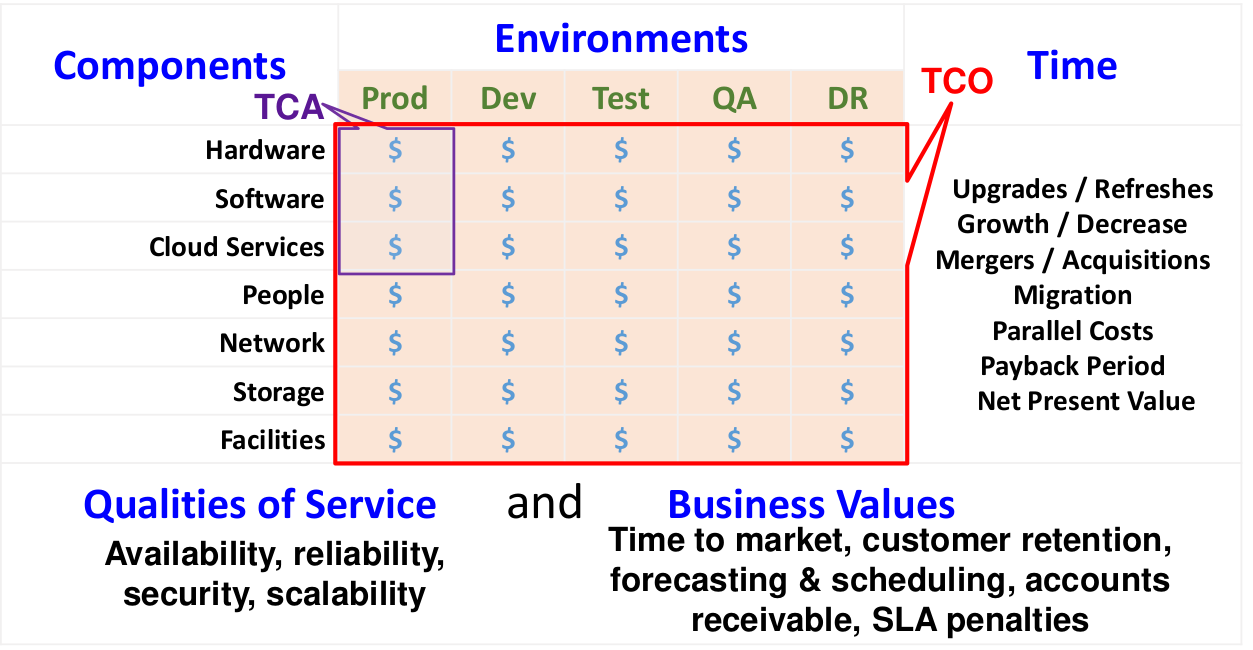
\includegraphics[scale=0.2]{images/TCO-TCA.png}\\
\caption{TCO vs TCA}
\end{figure} 
ogni applicazione ha dei costi legati ad hardware, software, servizi cloud e questi sono i TCA (Total Cost of Acquisition). Vanno anche considerati i costi di gestione del server e dell'applicazione, tipicamente per ogni 30 server occorre un IT admin (anche se non è una sola persona, possono essere anche di più che poi completano un full time equivalent, ovvero 40h/sett).\\ Bisogna anche considerare altre voci di costo, che sono presenti anche per tutti gli altri ambienti e di tutti i requisiti introdotti prima, come anche dei business values e del tempo: una cosa è il costo di acquisto, ma poi nel tempo dovrò fare degli upgrades software, refresh hardware e quindi tipicamente il TCO si fa su una finestra di 5 anni; spesso il refresh cycle viene stabilito nell'azienda: sul totale dei server, se ne cambieranno periodicamente (non per forza tutti insieme) un certo numero. Spendere decine di milioni per mettere su un ambiente Enterprise è abbastanza comune: a seconda della scelta di avere scale up o scale out ci saranno costi diversi, ma tipicamente il costo di scale out è maggiore; inoltre, la parte che ormai ha un costo predominante del TCO è quella del software come anche il costo del disater recovery (che deve mettere insieme i costi di hardware, software etc... che copre non per forza tutti gli stessi servizi dell'ambiente main site).
\subsection{Rack - z15}
In un ambiente Enterprise, rispetto ad un ambiente x86, posso avere un singolo rack (evoluzione dei mainframe), ne esistono due versioni:
\begin{itemize}
\item z15, ultima versione. Possono girarvi n sistemi operativi
\item LinuxONE, mainframe dedicata la mondo Linux
\end{itemize}
\subsubsection{Hardware z15}
L'hardware viene visto come un data-center in una scatola, composto da n server più i sistemi di storage, networking etc..., è stato progettato per virtualizzare e condividere le risorse: sopra il firmware di virtualizzazione gira lo z/VM, che crea VM dal punto di vista hardware (hypervisor di tipo 1).\\ Su ogni z/VM gira un z/OS e possono essere differenti, o anche un altro hypervisor.Ci sono diverse tipologie di processori:
\begin{itemize}
\item di tipo generale (equivalente delle CPU)
\item alcuni dedicati a fare dei compiti specifici (ad esempio per la gestione dell'I/O)
\item processori dedicati all'accoppiamento di due macchine, per farla sembrare una singola
\item zaaP, ottimizzati per eseguire il codice Java (ottimizzare la garbage collection etc...), sono una configurazione particolare di quelli generali
\item spare processor, di scorta. In questo modo se un'altra delle CPU fallisce, questi entrano in gioco
\end{itemize}
\paragraph{LPAR}suddivisione del sistema z in una macchina logica che viene configurata su misura, viene fatta anche dal punto di vista hardware per efficienza. Le LPAR sono isolate dal punto di vista hardware, in modo che in caso di guasti le altre LPAR rimangono su. Siccome il server z è configurato con diversi LPAR, riesce a stare su per decine di anni (senza fare reboot), possono condividere hardware, ma la memoria deve essere isolata.\\
\paragraph{RAIM - memory sparing}si usano memorie RAIM (Redudant Array Indipendent Memory): ci sono più banchi di memoria, in modo che se uno si rompe ce n'è un altro che ha i dati disponibili. Il RAIM prende il 20\% della memoria diposnibile, e versioni non RAIM non sono disponibili su macchine simili.\\ Lo z15 contiene fino a 108 core a 5.2GHz, fino a 40TB di memoria configurabile, offre anche retro compatibilità fino agli anni 60. Si parla di un "data center in a box", i costi saranno molto elevati.
\subsubsection{Confronto x86}
Sicuramente per avere le stesse prestazioni devo avere molteplici server, e abbiamo visto che al crescere dei server crescono anche i problemi in termini di availability, security etc...
\subsection{Gestione dei picchi di carico}
Un altro problema importante da gestire è calibrare un sistema per gestire i picchi di carico: fare over-provisioning è una soluzione tipica, ma c'è un grande spreco di risorse, quindi prezzi più alti così come anche consumi più alti.\\ Uno degli approcci è quello di usare un ambiente cloud, per sfruttarne l'elasticità, tipicamente per una Enterprise si configura un ambiente dedicato in base al tipo di applicazione. L'utilizzazione tipica dei server sta intorno al 20\%, sotto alto utilizzo siamo introno al 30\%, questo in base allo statistical multiplexing model: in base alla media, posso avere picchi differenti in base all'applicazione. Esistono diversi studi dello statistical multiplexing per cui se mettiamo su un servizio su un server, la probabilità che tutti i server abbiano un picco di richieste è molto bassa (utilizzazione pari ad 1), ci sono diversi server di tipo Enterprise in cui la distanza fra picco e media è bassa.\\ Queste macchine inoltre sono state pensate per lavorare ad utilizzazione al 100\%, il sistema operativo è abituato a girare all' 80-90\% e tutto ciò porta ad avere un utilizzo delle risorse molto ottimizzato.
\subsection{Case study - TCO su 5 anni}
Come abbiamo visto, per un analisi completa del TCO, dobbiamo avere una visione completa su tutti i componenti dell'applicazione, non solo in termini hardware e software ma anche per le persone etc... e questo per tutti i possibili ambienti.\\ A seconda degli anni, ci sono costi più preponderanti rispetto ad altri etc...\\ Per effettuare un TCO, occorrono 4 passi principali:
\begin{itemize}
\item Analizzare lo UC e capire il workload, solitamente si effettua parlando con il cliente. Occorre capire sia la media che i picchi del workload, misurato in TPS (transaction per seconds): non avviene così spesso che l'analisi venga fatta prima di mettere in esercizio un sistema, nel caso in cui l'ambiente sia già in esercizio, i valori si possono inferire dal sistema già in esercizio. Si ottengono dei report su una finestra minima di 1 mese per ricavare i valori, altrimenti occorrerà fare delle stime o delle ipotesi.
\item Valutazione e dimensionamento della piattaforma per permettere di supportare il workload, quindi ad esempio capire la taglia del server su cui deployare l'ambiente:
\begin{itemize}
\item taglia dell'ambiente di produzione, considerando i requisiti di HA
\item sizing di tutti gli altri ambienti: Dev e Test, Pre-prod, DR
\end{itemize}
il sizing del distaster recovery è molto interessante, bisogna trovare il compromesso giusto. Occorre inoltre confrontare scale up con scale down
\item valutazione dei costi, analisi del TCO
\item descrizione con grafici, dati, tabelle etc.. facendo riferimento ai dati di input
\end{itemize}
\subsubsection{Sizing}
Fare un sizing preciso è complesso: occorre analizzare i dati, facendo analisi tecnica dell'hardware e del software, la tipologia di VM e di hypervisor etc...\\ Partiamo da un'ipotesi semplificata: il numero di core di un ambiente Enterprise è almeno 17 volte minore di un ambiente x86. Partiamo da una ipotesi consolidata (slides)\\ A questo punto, andrebbe progettata l'architettura tecnica: spesso esiste già, quindi va modificata ed evoluta (N.B: l'ambiente di pre-prod dovrebbe avere la stessa taglia del prod). Si parla più che altro di core: è possibile avere un server con 12 core, o uno equivalente che ne ha 24 l'importante è la capacità elaborativa.\\ esempio 1: situazione active passive, dove mantengo dei core per il DR da parte, per sopperire a disastri.\\ esempio 2: active active (vedi video).\\ In LinuxONE: \\ esempio1: posso tenere nel sito 24-75 CBU (core di backup)\\ esempio 2: ho abbastanza CBU per poter coprire la pre-prod e la prod, con un ambiente di sviluppo e test più piccoli. LinuxONE: una delle due architetture z della IBM, su cui girano solo software di tipo Linxu\footnote{distro supportate: Red Hat, Suse, Ubuntu}.
\subsubsection{Costi}
Occorre valutare diversi costi:
\begin{itemize}
\item Il software deve girare su un software stack, il tipico prevede:
\begin{itemize}
\item OS
\item VM
\item Application server: oltre al classico software, permette di poter gestire differenti transazioni in parallelo. Ho il software che coordina le chiamate alle transazioni, da smistare sui vari server.
\item DB
\item data replication tool
\item tool di monitoring
\item security tools
\end{itemize}
per tutti, occorre conoscere diversi prezzi.
\end{itemize}
Gli altri costi di cui si tiene conto sono:
\begin{itemize}
\item costi per le persone, che devono manutenere i server. Un full-time equivalent (una persona assegnata a tempo pieno) può fornire supporto fino a 30 server. Occorre considerare anche i fully loaded cost, non solo il salario: oltre a quello ed alle tasse, ci sono una serie di costi come l'ufficio, il manager del team etc...
\item costi di rete: tipicamente, per ambiente Enterprise è in media 7000\$ per server
\item costi di facilities: affitto del data center, costi di elettricità
\end{itemize}
un altro elemento che sta diventando importante è il carbon footprint, ovvero l'emissione di $CO_{2}$ del data center.
\subsection{Use case: transazione con carta di credito di una banca}
Ogni acquisto del cliente va registrato sui server, occorre verificare un sacco di cose per poter completare e validare una transazione. Una transazione concettuale è fatta di molteplici transazioni IT, assumiamo che un core x86 possa effettuare 20 TPS, intese come transazioni concettuali.\\ Importante: il costo per core conta anche quelli spare, quindi se non attivi dono soldi "buttati".\\ Per il software: a seconda del utilizzo può cambiare il prezzo: ad esempio per l'ambiente di production può avere un costo maggiore di quello di dev.\\ Tipicamente: sul LinuxONE è possibile avere diversi carichi sulle CPU, perché sono progettati per lavorare al 90-95 \% di utilizzazione, mentre per x86 non è così (se il carico cresce troppo, si rischia di violare lo SLA).
\section{Feedback sul case study}
Considerazioni:
\begin{itemize}
\item difficoltà nel trovare prezzi per software
\item difficoltà nel determinare HA e DR
\item se usare come valore per le TPS la media o i picchi
\end{itemize}
\paragraph{Gestione dei picchi di TPS}per la gestione dei picchi, quando si calibra un sistema con un tool come foglio Excel, calibriamo il sistema per gestire quel numero di TPS: il numero di core ottenuto soddisfa un carico di 2000 TPS, se ne arrivano di più ne occorrono di più. Quindi, metto le TPS di picco in modo tale da poter gestire i picchi e sicuramente la media. La richiesta di carico sarà dettata dalla domanda, se riesco ad essere elastico posso riuscire a seguire la curva per avere il minimo dello spreco.

\paragraph{Spare cores}concetto solo del mondo LinuxONE, nel mondo x86 ci sono spare servers. Quindi o i core sono attivi o non lo sono, il costo del modello nel foglio Excel conta solo i core non attivi. Nel creare un LPAR, è come creare un server fisico con quel numero di core.
\paragraph{DR}l'ambiente di DR può essere attivo-attivo o attivo-passivo, ma questo dipende dalle considerazioni: se quando è passivo i server sono spenti, allora potrebbe non esserci costo per il software. In realtà nessuno lascia il DR completamente spento, inoltre quando si acquistano risorse conviene prenderle da più fornitori, per evitare che in caso di disastro si venga bloccati.
\paragraph{Sizing}spesso per il sizing si segue un processo iterativo: si parla col cliente per poter capire, in base al budget, come regolarsi sul dimensionamento dell'architettura.
\paragraph{Statistical multiplexing}esiste un modello di statistical multiplexing, molto studiato in TLC: se consolido vari workload su un ambiente virtualizzato, quindi se ho un servente potente, più il numero di utilizzatori cresce e più il servente avrà un carico che sarà una media più o meno costante. La telefonia analogica prevedeva che nel momento in cui veniva composto il numero, la chiamata arrivava in centrale e questa stabiliva una connessione punto-punto tra il chiamante ed il ricevente. Quindi, la connessione, perfetta richiedeva una topologia a stella ma questo prevedeva un costo che cresce come $O(n^2)$. In realtà, veniva messo un numero limitato, circa quanto il numero medio di chiamate effettuate in una giornata. Quindi, più il servente cresce, più è poco probabile che i picchi, quando ci sono molti serventi, siano poco limitati intorno alla media. Quindi, se un server può supportare un certo numero di VM, ogni VM farà girare un software che gestirà un aspetto dell'applicazione, avrà una media di utilizzo molto grande ma le oscillazioni dei picchi sono molto più vicine alla media. Quindi, se un server può supportare un carico di 1000 VM, la media ed i picchi sono circa uguali. Quindi, nel mondo LinuxONE, posso considerare i calcoli sulla media, mentre nel mondo x86 devo considerare i picchi. Il discorso funziona quando la richiesta di servizio è incredibilmente eterogenea, ma anche quando le TPS sono eterogenee. Inoltre, in questo modo è possibile arrivare ad una server utilization del 70\%, in modo da sfruttare bene le macchine. Il sizing è complesso:
\begin{itemize}
\item occorre conoscere bene il workload
\item sapere bene i picchi
\item etc ...
\end{itemize}
\paragraph{Gestione dell'HA}almeno uno o due server di backup, fare un analisi per l'HA di 5-6-7 "9" richiede un'analisi molto più sofisticata, le considerazioni fanno riferimento al grado di ridondanza che si ha.
\paragraph{Costo di licenza}il licesing model più presente è per core, è realistico che il prezzo sia indipendente dal tipo di core? Il core LinuxONE è molto più performante di quello x86, esistono dei correttivi per il prezzo:
\begin{itemize}
\item scontistica: al crescere del numero di core, lo sconto aumenta
\item fattore correttivo: per sopperire al fatto che alcuni core sono più economici di altri, questo fattore aiuta. Per i DB, molto spesso c'è un fattore dello 0.5, ovvero nel mondo x86 serve una licenza per 2 core, mentre in LinuxONE il rapporto è 1-a-1. Le VPC, che corrispondono a diversi core per i diversi ambienti, ci sistemano le cose.
\end{itemize}
Sarebbe possibile spalmare nel tempo l'acquisto dell'hardware, in modo che a seconda della crescita del business crescerà l'hardware della percentuale di crescita.
\subsection{Q\&A}
\paragraph{Sizing in base allo statistical multiplexing} Per lo statistical multiplexing, i mainframe LinuxONE possono essere consolidati a lavorare su diversi workload in modo da spingere l'utilizzazione al 70-80\%, mentre per sistemi x86 questo non è possibile, in quanto sono pensati per lavorare con un singolo workload. Quindi, una calibrazione più reale del sistema andrebbe fatta considerando:
\begin{itemize}
\item la media delle TPS per LinuxONE
\item i picchi di carico per x86
\end{itemize}
inoltre, in analisi di TCO reali occorre anche fare riferimento all'utilizzazione media per andare a fare un dimensionamento più accurato, il che rende il tutto molto più complesso.
\paragraph{NFR-6}nel NFR-6 veniva richiesto di effettuare un round completo di testing stressando il sistema ai picchi di carico. Per fare ciò, è necessario avere un ambiente di pre-produzione che abbia la stessa taglia dell'ambiente di produzione, quindi equivale a dire che pre prod = 100\% prod.\\ Spesso capita di calibrare il sistema per i FR e di fare stress test solo per la media dei carichi e non per i picchi.
\end{document}
